\section{Modeling and Managing ATSs - The CATSM Problem} 

% ==================///==================///==================///
\begin{frame}{How to tackle them?}
	By observing what we have. \\
	
	\vspace{0.5cm}
	\begin{itemize}
		\item Road Network
		\item Vehicles
		\item Requests
	\end{itemize}
	\vspace{0.5cm}
	$\rightarrow$ Creating a vehicle-centric model of the ATS to solve the challenges.
\end{frame}

% ==================///==================///==================///
\begin{frame}{Modeling the Road Network}
	Using a uni-directed graph $\mathcal{G} = \langle \mathcal{V}, \mathcal{E} \rangle$, where $\mathcal{V}$ represents the set of vertices (locations) and $\mathcal{E} \subseteq \mathcal{V} \times \mathcal{V}$ represents the edges (roads).
	\vspace{0.5cm}
	\begin{itemize}
		\item Each edge is associated with multiple metrics (e.g., distance $d: \mathcal{E} \rightarrow \mathbb{R}_{\geq 0}$).
		\begin{itemize}
			\item[ ] $\Rightarrow$ Artificial limit on number of vehicles at each time
		\end{itemize}
		\item Nodes can be of two types: charging ($\mathcal{V}_c$) and normal ($\mathcal{V}_n$) nodes.
		\item Charging nodes using ad-hoc charging profile models.
	\end{itemize}
\end{frame}


% ==================///==================///==================///

%\begin{frame}{Charging Profiles}
%	 	\vspace{0.1cm}
%	AV batteries modeled as tuple  $\mathcal{T}_a =\langle Q_a, I^b_a, R^-_a, R^+_a,\theta_a\rangle$. \\
%	Using the CC-CV (Constant current - Constant Voltage) scheme. 
%	\vspace{0.1cm}
%	\begin{figure}[th]
	
	\begin{subfigure}{0.43\linewidth}
		\centering
		\resizebox{1\textwidth}{!}{
			\begin{tikzpicture}
				\begin{axis}[
					xlabel={t},
					ylabel={B(t)},
					%legend style={at={(1.05,1)},anchor=north west},
					ymajorgrids=true,
					grid style=dashed,
					thick,
					ymin=-1,
					ymax = 101, 
					thick,
					yticklabel style={color=viridisgreencolor}, 
					title={$R^+ = 1, \theta = 0.6, b = 60.0, \tau = 33.3$}
					]
					\addplot[color = viridisgreencolor]
					coordinates {
						(0.0, 0.0) (0.15015015015015015, 0.15015015015015015) (0.3003003003003003, 0.3003003003003003) (0.45045045045045046, 0.45045045045045046) (0.6006006006006006, 0.6006006006006006) (0.7507507507507507, 0.7507507507507507) (0.9009009009009009, 0.9009009009009009) (1.0510510510510511, 1.0510510510510511) (1.2012012012012012, 1.2012012012012012) (1.3513513513513513, 1.3513513513513513) (1.5015015015015014, 1.5015015015015014) (1.6516516516516517, 1.6516516516516517) (1.8018018018018018, 1.8018018018018018) (1.951951951951952, 1.951951951951952) (2.1021021021021022, 2.1021021021021022) (2.2522522522522523, 2.2522522522522523) (2.4024024024024024, 2.4024024024024024) (2.5525525525525525, 2.5525525525525525) (2.7027027027027026, 2.7027027027027026) (2.8528528528528527, 2.8528528528528527) (3.003003003003003, 3.003003003003003) (3.1531531531531534, 3.1531531531531534) (3.3033033033033035, 3.3033033033033035) (3.4534534534534536, 3.4534534534534536) (3.6036036036036037, 3.6036036036036037) (3.7537537537537538, 3.7537537537537538) (3.903903903903904, 3.903903903903904) (4.054054054054054, 4.054054054054054) (4.2042042042042045, 4.2042042042042045) (4.354354354354355, 4.354354354354355) (4.504504504504505, 4.504504504504505) (4.654654654654655, 4.654654654654655) (4.804804804804805, 4.804804804804805) (4.954954954954955, 4.954954954954955) (5.105105105105105, 5.105105105105105) (5.255255255255255, 5.255255255255255) (5.405405405405405, 5.405405405405405) (5.555555555555555, 5.555555555555555) (5.7057057057057055, 5.7057057057057055) (5.8558558558558556, 5.8558558558558556) (6.006006006006006, 6.006006006006006) (6.156156156156157, 6.156156156156157) (6.306306306306307, 6.306306306306307) (6.456456456456457, 6.456456456456457) (6.606606606606607, 6.606606606606607) (6.756756756756757, 6.756756756756757) (6.906906906906907, 6.906906906906907) (7.057057057057057, 7.057057057057057) (7.207207207207207, 7.207207207207207) (7.357357357357357, 7.357357357357357) (7.5075075075075075, 7.5075075075075075) (7.657657657657658, 7.657657657657658) (7.807807807807808, 7.807807807807808) (7.957957957957958, 7.957957957957958) (8.108108108108109, 8.108108108108109) (8.258258258258259, 8.258258258258259) (8.408408408408409, 8.408408408408409) (8.558558558558559, 8.558558558558559) (8.70870870870871, 8.70870870870871) (8.85885885885886, 8.85885885885886) (9.00900900900901, 9.00900900900901) (9.15915915915916, 9.15915915915916) (9.30930930930931, 9.30930930930931) (9.45945945945946, 9.45945945945946) (9.60960960960961, 9.60960960960961) (9.75975975975976, 9.75975975975976) (9.90990990990991, 9.90990990990991) (10.06006006006006, 10.06006006006006) (10.21021021021021, 10.21021021021021) (10.36036036036036, 10.36036036036036) (10.51051051051051, 10.51051051051051) (10.66066066066066, 10.66066066066066) (10.81081081081081, 10.81081081081081) (10.96096096096096, 10.96096096096096) (11.11111111111111, 11.11111111111111) (11.26126126126126, 11.26126126126126) (11.411411411411411, 11.411411411411411) (11.561561561561561, 11.561561561561561) (11.711711711711711, 11.711711711711711) (11.861861861861861, 11.861861861861861) (12.012012012012011, 12.012012012012011) (12.162162162162163, 12.162162162162163) (12.312312312312313, 12.312312312312313) (12.462462462462463, 12.462462462462463) (12.612612612612613, 12.612612612612613) (12.762762762762764, 12.762762762762764) (12.912912912912914, 12.912912912912914) (13.063063063063064, 13.063063063063064) (13.213213213213214, 13.213213213213214) (13.363363363363364, 13.363363363363364) (13.513513513513514, 13.513513513513514) (13.663663663663664, 13.663663663663664) (13.813813813813814, 13.813813813813814) (13.963963963963964, 13.963963963963964) (14.114114114114114, 14.114114114114114) (14.264264264264265, 14.264264264264265) (14.414414414414415, 14.414414414414415) (14.564564564564565, 14.564564564564565) (14.714714714714715, 14.714714714714715) (14.864864864864865, 14.864864864864865) (15.015015015015015, 15.015015015015015) (15.165165165165165, 15.165165165165165) (15.315315315315315, 15.315315315315315) (15.465465465465465, 15.465465465465465) (15.615615615615615, 15.615615615615615) (15.765765765765765, 15.765765765765765) (15.915915915915916, 15.915915915915916) (16.066066066066067, 16.066066066066067) (16.216216216216218, 16.216216216216218) (16.366366366366368, 16.366366366366368) (16.516516516516518, 16.516516516516518) (16.666666666666668, 16.666666666666668) (16.816816816816818, 16.816816816816818) (16.966966966966968, 16.966966966966968) (17.117117117117118, 17.117117117117118) (17.26726726726727, 17.26726726726727) (17.41741741741742, 17.41741741741742) (17.56756756756757, 17.56756756756757) (17.71771771771772, 17.71771771771772) (17.86786786786787, 17.86786786786787) (18.01801801801802, 18.01801801801802) (18.16816816816817, 18.16816816816817) (18.31831831831832, 18.31831831831832) (18.46846846846847, 18.46846846846847) (18.61861861861862, 18.61861861861862) (18.76876876876877, 18.76876876876877) (18.91891891891892, 18.91891891891892) (19.06906906906907, 19.06906906906907) (19.21921921921922, 19.21921921921922) (19.36936936936937, 19.36936936936937) (19.51951951951952, 19.51951951951952) (19.66966966966967, 19.66966966966967) (19.81981981981982, 19.81981981981982) (19.96996996996997, 19.96996996996997) (20.12012012012012, 20.12012012012012) (20.27027027027027, 20.27027027027027) (20.42042042042042, 20.42042042042042) (20.57057057057057, 20.57057057057057) (20.72072072072072, 20.72072072072072) (20.87087087087087, 20.87087087087087) (21.02102102102102, 21.02102102102102) (21.17117117117117, 21.17117117117117) (21.32132132132132, 21.32132132132132) (21.47147147147147, 21.47147147147147) (21.62162162162162, 21.62162162162162) (21.77177177177177, 21.77177177177177) (21.92192192192192, 21.92192192192192) (22.07207207207207, 22.07207207207207) (22.22222222222222, 22.22222222222222) (22.37237237237237, 22.37237237237237) (22.52252252252252, 22.52252252252252) (22.67267267267267, 22.67267267267267) (22.822822822822822, 22.822822822822822) (22.972972972972972, 22.972972972972972) (23.123123123123122, 23.123123123123122) (23.273273273273272, 23.273273273273272) (23.423423423423422, 23.423423423423422) (23.573573573573572, 23.573573573573572) (23.723723723723722, 23.723723723723722) (23.873873873873872, 23.873873873873872) (24.024024024024023, 24.024024024024023) (24.174174174174176, 24.174174174174176) (24.324324324324326, 24.324324324324326) (24.474474474474476, 24.474474474474476) (24.624624624624627, 24.624624624624627) (24.774774774774777, 24.774774774774777) (24.924924924924927, 24.924924924924927) (25.075075075075077, 25.075075075075077) (25.225225225225227, 25.225225225225227) (25.375375375375377, 25.375375375375377) (25.525525525525527, 25.525525525525527) (25.675675675675677, 25.675675675675677) (25.825825825825827, 25.825825825825827) (25.975975975975977, 25.975975975975977) (26.126126126126128, 26.126126126126128) (26.276276276276278, 26.276276276276278) (26.426426426426428, 26.426426426426428) (26.576576576576578, 26.576576576576578) (26.726726726726728, 26.726726726726728) (26.876876876876878, 26.876876876876878) (27.027027027027028, 27.027027027027028) (27.177177177177178, 27.177177177177178) (27.32732732732733, 27.32732732732733) (27.47747747747748, 27.47747747747748) (27.62762762762763, 27.62762762762763) (27.77777777777778, 27.77777777777778) (27.92792792792793, 27.92792792792793) (28.07807807807808, 28.07807807807808) (28.22822822822823, 28.22822822822823) (28.37837837837838, 28.37837837837838) (28.52852852852853, 28.52852852852853) (28.67867867867868, 28.67867867867868) (28.82882882882883, 28.82882882882883) (28.97897897897898, 28.97897897897898) (29.12912912912913, 29.12912912912913) (29.27927927927928, 29.27927927927928) (29.42942942942943, 29.42942942942943) (29.57957957957958, 29.57957957957958) (29.72972972972973, 29.72972972972973) (29.87987987987988, 29.87987987987988) (30.03003003003003, 30.03003003003003) (30.18018018018018, 30.18018018018018) (30.33033033033033, 30.33033033033033) (30.48048048048048, 30.48048048048048) (30.63063063063063, 30.63063063063063) (30.78078078078078, 30.78078078078078) (30.93093093093093, 30.93093093093093) (31.08108108108108, 31.08108108108108) (31.23123123123123, 31.23123123123123) (31.38138138138138, 31.38138138138138) (31.53153153153153, 31.53153153153153) (31.68168168168168, 31.68168168168168) (31.83183183183183, 31.83183183183183) (31.98198198198198, 31.98198198198198) (32.132132132132135, 32.132132132132135) (32.28228228228228, 32.28228228228228) (32.432432432432435, 32.432432432432435) (32.58258258258258, 32.58258258258258) (32.732732732732735, 32.732732732732735) (32.88288288288288, 32.88288288288288) (33.033033033033036, 33.033033033033036) (33.18318318318318, 33.18318318318318) (33.333333333333336, 33.333333333333336) (33.48348348348348, 33.48348348348348) (33.633633633633636, 33.633633633633636) (33.78378378378378, 33.78378378378378) (33.933933933933936, 33.933933933933936) (34.08408408408408, 34.08408408408408) (34.234234234234236, 34.234234234234236) (34.38438438438438, 34.38438438438438) (34.53453453453454, 34.53453453453454) (34.68468468468468, 34.68468468468468) (34.83483483483484, 34.83483483483484) (34.98498498498498, 34.98498498498498) (35.13513513513514, 35.13513513513514) (35.28528528528528, 35.28528528528528) (35.43543543543544, 35.43543543543544) (35.585585585585584, 35.585585585585584) (35.73573573573574, 35.73573573573574) (35.885885885885884, 35.885885885885884) (36.03603603603604, 36.03603603603604) (36.186186186186184, 36.186186186186184) (36.33633633633634, 36.33633633633634) (36.486486486486484, 36.486486486486484) (36.63663663663664, 36.63663663663664) (36.786786786786784, 36.786786786786784) (36.93693693693694, 36.93693693693694) (37.087087087087085, 37.087087087087085) (37.23723723723724, 37.23723723723724) (37.387387387387385, 37.387387387387385) (37.53753753753754, 37.53753753753754) (37.687687687687685, 37.687687687687685) (37.83783783783784, 37.83783783783784) (37.987987987987985, 37.987987987987985) (38.13813813813814, 38.13813813813814) (38.288288288288285, 38.288288288288285) (38.43843843843844, 38.43843843843844) (38.58858858858859, 38.58858858858859) (38.73873873873874, 38.73873873873874) (38.88888888888889, 38.88888888888889) (39.03903903903904, 39.03903903903904) (39.18918918918919, 39.18918918918919) (39.33933933933934, 39.33933933933934) (39.48948948948949, 39.48948948948949) (39.63963963963964, 39.63963963963964) (39.78978978978979, 39.78978978978979) (39.93993993993994, 39.93993993993994) (40.090090090090094, 40.090090090090094) (40.24024024024024, 40.24024024024024) (40.390390390390394, 40.390390390390394) (40.54054054054054, 40.54054054054054) (40.690690690690694, 40.690690690690694) (40.84084084084084, 40.84084084084084) (40.990990990990994, 40.990990990990994) (41.14114114114114, 41.14114114114114) (41.291291291291294, 41.291291291291294) (41.44144144144144, 41.44144144144144) (41.591591591591595, 41.591591591591595) (41.74174174174174, 41.74174174174174) (41.891891891891895, 41.891891891891895) (42.04204204204204, 42.04204204204204) (42.192192192192195, 42.192192192192195) (42.34234234234234, 42.34234234234234) (42.492492492492495, 42.492492492492495) (42.64264264264264, 42.64264264264264) (42.792792792792795, 42.792792792792795) (42.94294294294294, 42.94294294294294) (43.093093093093096, 43.093093093093096) (43.24324324324324, 43.24324324324324) (43.393393393393396, 43.393393393393396) (43.54354354354354, 43.54354354354354) (43.693693693693696, 43.693693693693696) (43.84384384384384, 43.84384384384384) (43.993993993993996, 43.993993993993996) (44.14414414414414, 44.14414414414414) (44.294294294294296, 44.294294294294296) (44.44444444444444, 44.44444444444444) (44.5945945945946, 44.5945945945946) (44.74474474474474, 44.74474474474474) (44.8948948948949, 44.8948948948949) (45.04504504504504, 45.04504504504504) (45.1951951951952, 45.1951951951952) (45.34534534534534, 45.34534534534534) (45.4954954954955, 45.4954954954955) (45.645645645645644, 45.645645645645644) (45.7957957957958, 45.7957957957958) (45.945945945945944, 45.945945945945944) (46.0960960960961, 46.0960960960961) (46.246246246246244, 46.246246246246244) (46.3963963963964, 46.3963963963964) (46.546546546546544, 46.546546546546544) (46.6966966966967, 46.6966966966967) (46.846846846846844, 46.846846846846844) (46.996996996997, 46.996996996997) (47.147147147147145, 47.147147147147145) (47.2972972972973, 47.2972972972973) (47.447447447447445, 47.447447447447445) (47.5975975975976, 47.5975975975976) (47.747747747747745, 47.747747747747745) (47.8978978978979, 47.8978978978979) (48.048048048048045, 48.048048048048045) (48.1981981981982, 48.1981981981982) (48.34834834834835, 48.34834834834835) (48.4984984984985, 48.4984984984985) (48.64864864864865, 48.64864864864865) (48.7987987987988, 48.7987987987988) (48.94894894894895, 48.94894894894895) (49.0990990990991, 49.0990990990991) (49.24924924924925, 49.24924924924925) (49.3993993993994, 49.3993993993994) (49.54954954954955, 49.54954954954955) (49.6996996996997, 49.6996996996997) (49.84984984984985, 49.84984984984985) (50.0, 50.0) (50.150150150150154, 50.150150150150154) (50.3003003003003, 50.3003003003003) (50.450450450450454, 50.450450450450454) (50.6006006006006, 50.6006006006006) (50.750750750750754, 50.750750750750754) (50.9009009009009, 50.9009009009009) (51.051051051051054, 51.051051051051054) (51.2012012012012, 51.2012012012012) (51.351351351351354, 51.351351351351354) (51.5015015015015, 51.5015015015015) (51.651651651651655, 51.651651651651655) (51.8018018018018, 51.8018018018018) (51.951951951951955, 51.951951951951955) (52.1021021021021, 52.1021021021021) (52.252252252252255, 52.252252252252255) (52.4024024024024, 52.4024024024024) (52.552552552552555, 52.552552552552555) (52.7027027027027, 52.7027027027027) (52.852852852852855, 52.852852852852855) (53.003003003003, 53.003003003003) (53.153153153153156, 53.153153153153156) (53.3033033033033, 53.3033033033033) (53.453453453453456, 53.453453453453456) (53.6036036036036, 53.6036036036036) (53.753753753753756, 53.753753753753756) (53.9039039039039, 53.9039039039039) (54.054054054054056, 54.054054054054056) (54.2042042042042, 54.2042042042042) (54.354354354354356, 54.354354354354356) (54.5045045045045, 54.5045045045045) (54.65465465465466, 54.65465465465466) (54.8048048048048, 54.8048048048048) (54.95495495495496, 54.95495495495496) (55.1051051051051, 55.1051051051051) (55.25525525525526, 55.25525525525526) (55.4054054054054, 55.4054054054054) (55.55555555555556, 55.55555555555556) (55.705705705705704, 55.705705705705704) (55.85585585585586, 55.85585585585586) (56.006006006006004, 56.006006006006004) (56.15615615615616, 56.15615615615616) (56.306306306306304, 56.306306306306304) (56.45645645645646, 56.45645645645646) (56.606606606606604, 56.606606606606604) (56.75675675675676, 56.75675675675676) (56.906906906906904, 56.906906906906904) (57.05705705705706, 57.05705705705706) (57.207207207207205, 57.207207207207205) (57.35735735735736, 57.35735735735736) (57.507507507507505, 57.507507507507505) (57.65765765765766, 57.65765765765766) (57.80780780780781, 57.80780780780781) (57.95795795795796, 57.95795795795796) (58.10810810810811, 58.10810810810811) (58.25825825825826, 58.25825825825826) (58.40840840840841, 58.40840840840841) (58.55855855855856, 58.55855855855856) (58.70870870870871, 58.70870870870871) (58.85885885885886, 58.85885885885886) (59.00900900900901, 59.00900900900901) (59.15915915915916, 59.15915915915916) (59.30930930930931, 59.30930930930931) (59.45945945945946, 59.45945945945946) (59.60960960960961, 59.60960960960961) (59.75975975975976, 59.75975975975976) (59.90990990990991, 59.90990990990991) (60.06006006006006, 60.07200718125672) (60.210210210210214, 60.25145853162593) (60.36036036036036, 60.43010336043279) (60.510510510510514, 60.607945292487216) (60.66066066066066, 60.78498793630783) (60.810810810810814, 60.96123488419524) (60.96096096096096, 61.13668971230493) (61.111111111111114, 61.31135598071977) (61.26126126126126, 61.485237233522284) (61.411411411411414, 61.6583369988666) (61.56156156156156, 61.83065878904996) (61.711711711711715, 62.00220610058406) (61.86186186186186, 62.172982414265924) (62.012012012012015, 62.34299119524861) (62.16216216216216, 62.51223589311144) (62.312312312312315, 62.68071994193008) (62.46246246246246, 62.848446760346135) (62.612612612612615, 63.01541975163659) (62.76276276276276, 63.181642303782795) (62.912912912912915, 63.347117789539276) (63.06306306306306, 63.5118495665021) (63.213213213213216, 63.675840977177074) (63.36336336336336, 63.83909534904751) (63.513513513513516, 64.00161599464178) (63.66366366366366, 64.16340621160049) (63.813813813813816, 64.32446928274345) (63.96396396396396, 64.48480847613624) (64.11411411411412, 64.64442704515648) (64.26426426426427, 64.80332822855996) (64.41441441441441, 64.96151525054623) (64.56456456456456, 65.11899132082414) (64.71471471471472, 65.27575963467686) (64.86486486486487, 65.43182337302679) (65.01501501501501, 65.58718570250005) (65.16516516516516, 65.74184977549076) (65.31531531531532, 65.89581873022503) (65.46546546546547, 66.04909569082457) (65.61561561561561, 66.20168376737013) (65.76576576576576, 66.35358605596461) (65.91591591591592, 66.50480563879583) (66.06606606606607, 66.65534558419914) (66.21621621621621, 66.8052089467196) (66.36636636636636, 66.95439876717404) (66.51651651651652, 67.10291807271273) (66.66666666666667, 67.25076987688072) (66.81681681681681, 67.39795717967914) (66.96696696696696, 67.54448296762595) (67.11711711711712, 67.69035021381661) (67.26726726726727, 67.83556187798433) (67.41741741741743, 67.98012090656023) (67.56756756756756, 68.12403023273299) (67.71771771771772, 68.26729277650853) (67.86786786786787, 68.40991144476908) (68.01801801801803, 68.55188913133232) (68.16816816816817, 68.69322871701) (68.31831831831832, 68.83393306966644) (68.46846846846847, 68.97400504427671) (68.61861861861863, 69.1134474829845) (68.76876876876877, 69.25226321515989) (68.91891891891892, 69.3904550574567) (69.06906906906907, 69.52802581386969) (69.21921921921923, 69.66497827579133) (69.36936936936937, 69.8013152220686) (69.51951951951952, 69.93703941905929) (69.66966966966967, 70.07215362068811) (69.81981981981983, 70.20666056850266) (69.96996996996997, 70.34056299172889) (70.12012012012012, 70.47386360732673) (70.27027027027027, 70.60656512004499) (70.42042042042043, 70.73867022247632) (70.57057057057057, 70.87018159511186) (70.72072072072072, 71.00110190639565) (70.87087087087087, 71.13143381277871) (71.02102102102103, 71.26117995877301) (71.17117117117117, 71.39034297700503) (71.32132132132132, 71.51892548826932) (71.47147147147147, 71.64693010158153) (71.62162162162163, 71.77435941423147) (71.77177177177177, 71.90121601183569) (71.92192192192192, 72.02750246839008) (72.07207207207207, 72.15322134632203) (72.22222222222223, 72.27837519654234) (72.37237237237237, 72.40296655849714) (72.52252252252252, 72.52699796021932) (72.67267267267268, 72.65047191837984) (72.82282282282283, 72.77339093833876) (72.97297297297297, 72.89575751419619) (73.12312312312312, 73.01757412884277) (73.27327327327328, 73.13884325401008) (73.42342342342343, 73.25956735032088) (73.57357357357357, 73.3797488673389) (73.72372372372372, 73.49939024361868) (73.87387387387388, 73.61849390675494) (74.02402402402403, 73.73706227343186) (74.17417417417417, 73.85509774947216) (74.32432432432432, 73.97260272988595) (74.47447447447448, 74.08957959891919) (74.62462462462463, 74.20603073010214) (74.77477477477477, 74.32195848629759) (74.92492492492492, 74.4373652197487) (75.07507507507508, 74.55225327212676) (75.22522522522523, 74.66662497457875) (75.37537537537537, 74.78048264777456) (75.52552552552552, 74.89382860195417) (75.67567567567568, 75.0066651369744) (75.82582582582583, 75.11899454235574) (75.97597597597597, 75.23081909732865) (76.12612612612612, 75.34214107087992) (76.27627627627628, 75.45296272179866) (76.42642642642643, 75.56328629872206) (76.57657657657657, 75.67311404018122) (76.72672672672672, 75.78244817464635) (76.87687687687688, 75.8912909205721) (77.02702702702703, 75.99964448644259) (77.17717717717719, 76.10751107081612) (77.32732732732732, 76.21489286236991) (77.47747747747748, 76.3217920399444) (77.62762762762763, 76.42821077258753) (77.77777777777779, 76.53415121959873) (77.92792792792793, 76.6396155305727) (78.07807807807808, 76.74460584544309) (78.22822822822823, 76.84912429452586) (78.37837837837839, 76.95317299856258) (78.52852852852853, 77.05675406876333) (78.67867867867868, 77.1598696068497) (78.82882882882883, 77.2625217050973) (78.97897897897899, 77.36471244637832) (79.12912912912913, 77.46644390420371) (79.27927927927928, 77.5677181427653) (79.42942942942943, 77.66853721697767) (79.57957957957959, 77.76890317251981) (79.72972972972973, 77.86881804587671) (79.87987987987988, 77.9682838643806) (80.03003003003003, 78.06730264625216) (80.18018018018019, 78.16587640064137) (80.33033033033033, 78.26400712766839) (80.48048048048048, 78.36169681846407) (80.63063063063063, 78.45894745521039) (80.78078078078079, 78.55576101118062) (80.93093093093093, 78.65213945077944) (81.08108108108108, 78.74808472958276) (81.23123123123123, 78.84359879437737) (81.38138138138139, 78.9386835832005) (81.53153153153153, 79.0333410253791) (81.68168168168168, 79.12757304156901) (81.83183183183183, 79.22138154379391) (81.98198198198199, 79.31476843548415) (82.13213213213213, 79.40773561151533) (82.28228228228228, 79.50028495824681) (82.43243243243244, 79.59241835355986) (82.58258258258259, 79.68413766689596) (82.73273273273273, 79.77544475929453) (82.88288288288288, 79.86634148343082) (83.03303303303304, 79.95682968365347) (83.18318318318319, 80.04691119602191) (83.33333333333333, 80.13658784834362) (83.48348348348348, 80.22586146021126) (83.63363363363364, 80.31473384303956) (83.78378378378379, 80.40320680010205) (83.93393393393393, 80.49128212656765) (84.08408408408408, 80.57896160953722) (84.23423423423424, 80.66624702807958) (84.38438438438439, 80.75314015326786) (84.53453453453453, 80.83964274821527) (84.68468468468468, 80.92575656811096) (84.83483483483484, 81.01148336025555) (84.98498498498499, 81.0968248640967) (85.13513513513513, 81.1817828112643) (85.28528528528528, 81.26635892560569) (85.43543543543544, 81.35055492322051) (85.58558558558559, 81.43437251249571) (85.73573573573573, 81.51781339414003) (85.88588588588588, 81.60087926121864) (86.03603603603604, 81.6835717991874) (86.18618618618619, 81.76589268592713) (86.33633633633633, 81.8478435917776) (86.48648648648648, 81.9294261795715) (86.63663663663664, 82.01064210466802) (86.78678678678679, 82.0914930149867) (86.93693693693695, 82.17198055104055) (87.08708708708708, 82.25210634596962) (87.23723723723724, 82.33187202557399) (87.38738738738739, 82.41127920834673) (87.53753753753755, 82.49032950550685) (87.68768768768768, 82.56902452103193) (87.83783783783784, 82.6473658516907) (87.98798798798799, 82.72535508707531) (88.13813813813815, 82.80299380963385) (88.28828828828829, 82.88028359470212) (88.43843843843844, 82.95722601053592) (88.58858858858859, 83.03382261834263) (88.73873873873875, 83.11007497231301) (88.88888888888889, 83.18598461965271) (89.03903903903904, 83.26155310061367) (89.1891891891892, 83.3367819485253) (89.33933933933935, 83.41167268982572) (89.48948948948949, 83.48622684409264) (89.63963963963964, 83.56044592407423) (89.7897897897898, 83.63433143571977) (89.93993993993995, 83.70788487821028) (90.09009009009009, 83.78110774398888) (90.24024024024024, 83.8540015187911) (90.3903903903904, 83.926567681675) (90.54054054054055, 83.9988077050512) (90.69069069069069, 84.0707230547128) (90.84084084084084, 84.14231518986504) (90.990990990991, 84.21358556315494) (91.14114114114115, 84.28453562070078) (91.29129129129129, 84.35516680212146) (91.44144144144144, 84.42548054056569) (91.5915915915916, 84.49547826274107) (91.74174174174175, 84.56516138894304) (91.89189189189189, 84.63453133308369) (92.04204204204204, 84.7035895027205) (92.1921921921922, 84.77233729908481) (92.34234234234235, 84.84077611711032) (92.49249249249249, 84.90890734546139) (92.64264264264264, 84.97673236656118) (92.7927927927928, 85.04425255661975) (92.94294294294295, 85.11146928566193) (93.09309309309309, 85.17838391755515) (93.24324324324324, 85.24499781003712) (93.3933933933934, 85.31131231474336) (93.54354354354355, 85.37732877723465) (93.69369369369369, 85.44304853702428) (93.84384384384384, 85.50847292760531) (93.993993993994, 85.57360327647756) (94.14414414414415, 85.63844090517455) (94.29429429429429, 85.70298712929036) (94.44444444444444, 85.76724325850631) (94.5945945945946, 85.83121059661751) (94.74474474474475, 85.89489044155928) (94.89489489489489, 85.95828408543359) (95.04504504504504, 86.02139281453522) (95.1951951951952, 86.08421790937783) (95.34534534534535, 86.14676064471998) (95.49549549549549, 86.20902228959098) (95.64564564564564, 86.27100410731668) (95.7957957957958, 86.33270735554504) (95.94594594594595, 86.39413328627171) (96.09609609609609, 86.45528314586534) (96.24624624624624, 86.51615817509301) (96.3963963963964, 86.57675960914527) (96.54654654654655, 86.6370886776613) (96.6966966966967, 86.69714660475378) (96.84684684684684, 86.75693460903383) (96.996996996997, 86.8164539036356) (97.14714714714715, 86.87570569624104) (97.2972972972973, 86.93469118910426) (97.44744744744744, 86.993411579076) (97.5975975975976, 87.05186805762796) (97.74774774774775, 87.11006181087684) (97.8978978978979, 87.16799401960856) (98.04804804804805, 87.22566585930208) (98.1981981981982, 87.28307850015338) (98.34834834834835, 87.3402331070991) (98.4984984984985, 87.39713083984023) (98.64864864864865, 87.45377285286561) (98.7987987987988, 87.51016029547543) (98.94894894894895, 87.56629431180444) (99.0990990990991, 87.62217604084523) (99.24924924924925, 87.67780661647136) (99.3993993993994, 87.73318716746031) (99.54954954954955, 87.78831881751641) (99.6996996996997, 87.84320268529366) (99.84984984984985, 87.8978398844184) (100.0, 87.95223152351191) (100.15015015015015, 88.00637870621293) (100.30030030030031, 88.06028253120002) (100.45045045045045, 88.11394409221384) (100.6006006006006, 88.16736447807945) (100.75075075075075, 88.22054477272823) (100.90090090090091, 88.27348605522002) (101.05105105105105, 88.32618939976496) (101.2012012012012, 88.37865587574527) (101.35135135135135, 88.43088654773697) (101.50150150150151, 88.48288247553148) (101.65165165165165, 88.53464471415712) (101.8018018018018, 88.58617431390053) (101.95195195195195, 88.63747232032793) (102.10210210210211, 88.68853977430642) (102.25225225225225, 88.73937771202502) (102.4024024024024, 88.78998716501576) (102.55255255255256, 88.84036916017455) (102.70270270270271, 88.89052471978205) (102.85285285285285, 88.94045486152443) (103.003003003003, 88.99016059851397) (103.15315315315316, 89.03964293930966) (103.30330330330331, 89.08890288793764) (103.45345345345345, 89.13794144391157) (103.6036036036036, 89.18675960225296) (103.75375375375376, 89.2353583535113) (103.90390390390391, 89.28373868378415) (104.05405405405405, 89.33190157473723) (104.2042042042042, 89.37984800362423) (104.35435435435436, 89.42757894330677) (104.50450450450451, 89.47509536227398) (104.65465465465465, 89.5223982246623) (104.8048048048048, 89.56948849027496) (104.95495495495496, 89.61636711460149) (105.10510510510511, 89.66303504883705) (105.25525525525525, 89.70949323990179) (105.4054054054054, 89.75574263046009) (105.55555555555556, 89.8017841589396) (105.70570570570571, 89.84761875955033) (105.85585585585586, 89.89324736230358) (106.006006006006, 89.9386708930309) (106.15615615615616, 89.98389027340274) (106.30630630630631, 90.02890642094724) (106.45645645645646, 90.0737202490688) (106.6066066066066, 90.11833266706671) (106.75675675675676, 90.16274458015346) (106.90690690690691, 90.20695688947319) (107.05705705705707, 90.25097049211998) (107.2072072072072, 90.29478628115601) (107.35735735735736, 90.33840514562972) (107.50750750750751, 90.38182797059383) (107.65765765765767, 90.42505563712332) (107.8078078078078, 90.46808902233325) (107.95795795795796, 90.51092899939661) (108.10810810810811, 90.55357643756206) (108.25825825825827, 90.59603220217147) (108.4084084084084, 90.63829715467759) (108.55855855855856, 90.68037215266146) (108.70870870870871, 90.72225804984981) (108.85885885885887, 90.76395569613246) (109.009009009009, 90.80546593757941) (109.15915915915916, 90.84678961645822) (109.30930930930931, 90.88792757125091) (109.45945945945947, 90.92888063667105) (109.6096096096096, 90.96964964368073) (109.75975975975976, 91.01023541950735) (109.90990990990991, 91.05063878766046) (110.06006006006007, 91.09086056794845) (110.2102102102102, 91.13090157649519) (110.36036036036036, 91.17076262575655) (110.51051051051051, 91.21044452453697) (110.66066066066067, 91.24994807800576) (110.8108108108108, 91.28927408771355) (110.96096096096096, 91.32842335160848) (111.11111111111111, 91.36739666405241) (111.26126126126127, 91.40619481583704) (111.41141141141141, 91.44481859419997) (111.56156156156156, 91.48326878284065) (111.71171171171171, 91.52154616193629) (111.86186186186187, 91.55965150815769) (112.01201201201201, 91.59758559468499) (112.16216216216216, 91.6353491912234) (112.31231231231232, 91.67294306401875) (112.46246246246247, 91.71036797587311) (112.61261261261261, 91.74762468616021) (112.76276276276276, 91.78471395084088) (112.91291291291292, 91.82163652247837) (113.06306306306307, 91.85839315025362) (113.21321321321321, 91.89498457998049) (113.36336336336336, 91.93141155412087) (113.51351351351352, 91.96767481179975) (113.66366366366367, 92.00377508882019) (113.81381381381381, 92.03971311767832) (113.96396396396396, 92.07548962757812) (114.11411411411412, 92.11110534444627) (114.26426426426427, 92.14656099094687) (114.41441441441441, 92.18185728649607) (114.56456456456456, 92.21699494727672) (114.71471471471472, 92.25197468625288) (114.86486486486487, 92.28679721318426) (115.01501501501501, 92.32146323464066) (115.16516516516516, 92.3559734540163) (115.31531531531532, 92.39032857154403) (115.46546546546547, 92.42452928430967) (115.61561561561562, 92.45857628626602) (115.76576576576576, 92.49247026824702) (115.91591591591592, 92.52621191798173) (116.06606606606607, 92.55980192010831) (116.21621621621622, 92.59324095618788) (116.36636636636636, 92.6265297047184) (116.51651651651652, 92.65966884114837) (116.66666666666667, 92.69265903789062) (116.81681681681683, 92.72550096433584) (116.96696696696696, 92.75819528686628) (117.11711711711712, 92.79074266886921) (117.26726726726727, 92.82314377075039) (117.41741741741743, 92.85539924994742) (117.56756756756756, 92.8875097609432) (117.71771771771772, 92.91947595527911) (117.86786786786787, 92.95129848156824) (118.01801801801803, 92.9829779855086) (118.16816816816817, 93.01451510989618) (118.31831831831832, 93.045910494638) (118.46846846846847, 93.07716477676509) (118.61861861861863, 93.10827859044544) (118.76876876876877, 93.13925256699686) (118.91891891891892, 93.17008733489976) (119.06906906906907, 93.20078351980992) (119.21921921921923, 93.23134174457122) (119.36936936936937, 93.26176262922822) (119.51951951951952, 93.29204679103877) (119.66966966966967, 93.32219484448653) (119.81981981981983, 93.35220740129347) (119.96996996996997, 93.3820850704322) (120.12012012012012, 93.41182845813843) (120.27027027027027, 93.4414381679232) (120.42042042042043, 93.47091480058512) (120.57057057057057, 93.50025895422263) (120.72072072072072, 93.52947122424607) (120.87087087087087, 93.55855220338977) (121.02102102102103, 93.58750248172412) (121.17117117117117, 93.61632264666748) (121.32132132132132, 93.64501328299816) (121.47147147147147, 93.67357497286626) (121.62162162162163, 93.70200829580544) (121.77177177177177, 93.73031382874476) (121.92192192192192, 93.75849214602032) (122.07207207207207, 93.78654381938695) (122.22222222222223, 93.8144694180298) (122.37237237237237, 93.8422695085759) (122.52252252252252, 93.8699446551056) (122.67267267267268, 93.89749541916412) (122.82282282282283, 93.92492235977284) (122.97297297297297, 93.95222603344072) (123.12312312312312, 93.97940699417555) (123.27327327327328, 94.0064657934952) (123.42342342342343, 94.0334029804388) (123.57357357357357, 94.06021910157791) (123.72372372372372, 94.0869147010276) (123.87387387387388, 94.11349032045744) (124.02402402402403, 94.1399464991026) (124.17417417417417, 94.16628377377468) (124.32432432432432, 94.19250267887264) (124.47447447447448, 94.2186037463937) (124.62462462462463, 94.24458750594401) (124.77477477477477, 94.27045448474955) (124.92492492492492, 94.2962052076667) (125.07507507507508, 94.32184019719296) (125.22522522522523, 94.34735997347752) (125.37537537537538, 94.37276505433184) (125.52552552552552, 94.3980559552401) (125.67567567567568, 94.42323318936977) (125.82582582582583, 94.44829726758188) (125.97597597597598, 94.47324869844151) (126.12612612612612, 94.49808798822805) (126.27627627627628, 94.52281564094545) (126.42642642642643, 94.54743215833253) (126.57657657657658, 94.57193803987305) (126.72672672672672, 94.59633378280594) (126.87687687687688, 94.62061988213534) (127.02702702702703, 94.64479683064069) (127.17717717717719, 94.66886511888661) (127.32732732732732, 94.69282523523303) (127.47747747747748, 94.71667766584497) (127.62762762762763, 94.74042289470242) (127.77777777777779, 94.76406140361023) (127.92792792792793, 94.78759367220779) (128.07807807807808, 94.81102017797886) (128.22822822822823, 94.83434139626117) (128.3783783783784, 94.8575578002561) (128.52852852852854, 94.88066986103836) (128.6786786786787, 94.90367804756535) (128.82882882882882, 94.92658282668691) (128.97897897897897, 94.94938466315463) (129.12912912912913, 94.97208401963135) (129.27927927927928, 94.99468135670051) (129.42942942942943, 95.01717713287553) (129.5795795795796, 95.0395718046091) (129.72972972972974, 95.06186582630244) (129.8798798798799, 95.0840596503145) (130.03003003003002, 95.1061537269712) (130.18018018018017, 95.1281485045745) (130.33033033033033, 95.15004442941152) (130.48048048048048, 95.17184194576362) (130.63063063063063, 95.19354149591535) (130.7807807807808, 95.21514352016352) (130.93093093093094, 95.23664845682607) (131.0810810810811, 95.25805674225094) (131.23123123123122, 95.27936881082499) (131.38138138138137, 95.30058509498278) (131.53153153153153, 95.32170602521532) (131.68168168168168, 95.34273203007889) (131.83183183183183, 95.36366353620362) (131.981981981982, 95.38450096830222) (132.13213213213214, 95.4052447491786) (132.2822822822823, 95.42589529973644) (132.43243243243242, 95.44645303898766) (132.58258258258257, 95.46691838406105) (132.73273273273273, 95.48729175021062) (132.88288288288288, 95.50757355082412) (133.03303303303304, 95.52776419743134) (133.1831831831832, 95.54786409971253) (133.33333333333334, 95.56787366550664) (133.4834834834835, 95.5877933008197) (133.63363363363362, 95.60762340983295) (133.78378378378378, 95.62736439491111) (133.93393393393393, 95.6470166566105) (134.08408408408408, 95.66658059368723) (134.23423423423424, 95.68605660310521) (134.3843843843844, 95.70544508004427) (134.53453453453454, 95.72474641790815) (134.6846846846847, 95.74396100833246) (134.83483483483485, 95.7630892411927) (134.98498498498498, 95.78213150461208) (135.13513513513513, 95.80108818496947) (135.28528528528528, 95.8199596669072) (135.43543543543544, 95.83874633333885) (135.5855855855856, 95.85744856545708) (135.73573573573574, 95.8760667427413) (135.8858858858859, 95.89460124296542) (136.03603603603605, 95.91305244220547) (136.18618618618618, 95.93142071484726) (136.33633633633633, 95.94970643359399) (136.48648648648648, 95.96790996947377) (136.63663663663664, 95.98603169184716) (136.7867867867868, 96.0040719684147) (136.93693693693695, 96.02203116522436) (137.0870870870871, 96.03990964667891) (137.23723723723725, 96.05770777554338) (137.38738738738738, 96.07542591295238) (137.53753753753753, 96.09306441841751) (137.68768768768768, 96.11062364983451) (137.83783783783784, 96.12810396349063) (137.987987987988, 96.14550571407186) (138.13813813813815, 96.16282925467006) (138.2882882882883, 96.18007493679019) (138.43843843843845, 96.19724311035739) (138.58858858858858, 96.21433412372413) (138.73873873873873, 96.23134832367722) (138.88888888888889, 96.24828605544495) (139.03903903903904, 96.26514766270394) (139.1891891891892, 96.28193348758624) (139.33933933933935, 96.29864387068625) (139.4894894894895, 96.31527915106756) (139.63963963963965, 96.33183966626991) (139.78978978978978, 96.34832575231603) (139.93993993993993, 96.36473774371841) (140.0900900900901, 96.3810759734861) (140.24024024024024, 96.39734077313155) (140.3903903903904, 96.41353247267719) (140.54054054054055, 96.42965140066225) (140.6906906906907, 96.44569788414938) (140.84084084084085, 96.46167224873126) (140.99099099099098, 96.47757481853728) (141.14114114114113, 96.49340591624002) (141.2912912912913, 96.5091658630619) (141.44144144144144, 96.52485497878159) (141.5915915915916, 96.5404735817406) (141.74174174174175, 96.5560219888497) (141.8918918918919, 96.57150051559529) (142.04204204204206, 96.5869094760459) (142.19219219219218, 96.60224918285851) (142.34234234234233, 96.61751994728492) (142.4924924924925, 96.63272207917801) (142.64264264264264, 96.64785588699807) (142.7927927927928, 96.6629216778191) (142.94294294294295, 96.67791975733493) (143.0930930930931, 96.69285042986553) (143.24324324324326, 96.70771399836315) (143.39339339339338, 96.72251076441842) (143.54354354354354, 96.73724102826652) (143.6936936936937, 96.75190508879331) (143.84384384384384, 96.76650324354127) (143.993993993994, 96.78103578871566) (144.14414414414415, 96.79550301919046) (144.2942942942943, 96.8099052285144) (144.44444444444446, 96.82424270891687) (144.5945945945946, 96.83851575131389) (144.74474474474474, 96.85272464531397) (144.8948948948949, 96.86686967922404) (145.04504504504504, 96.88095114005525) (145.1951951951952, 96.89496931352882) (145.34534534534535, 96.90892448408184) (145.4954954954955, 96.92281693487301) (145.64564564564566, 96.93664694778843) (145.7957957957958, 96.95041480344732) (145.94594594594594, 96.96412078120761) (146.0960960960961, 96.9777651591718) (146.24624624624624, 96.9913482141924) (146.3963963963964, 97.00487022187771) (146.54654654654655, 97.0183314565973) (146.6966966966967, 97.03173219148763) (146.84684684684686, 97.04507269845759) (146.996996996997, 97.05835324819401) (147.14714714714714, 97.07157411016713) (147.2972972972973, 97.08473555263615) (147.44744744744744, 97.09783784265451) (147.5975975975976, 97.11088124607552) (147.74774774774775, 97.12386602755758) (147.8978978978979, 97.13679245056964) (148.04804804804806, 97.14966077739652) (148.1981981981982, 97.16247126914422) (148.34834834834834, 97.17522418574524) (148.4984984984985, 97.18791978596384) (148.64864864864865, 97.20055832740132) (148.7987987987988, 97.21314006650121) (148.94894894894895, 97.22566525855449) (149.0990990990991, 97.23813415770472) (149.24924924924926, 97.25054701695333) (149.3993993993994, 97.2629040881646) (149.54954954954954, 97.27520562207087) (149.6996996996997, 97.28745186827757) (149.84984984984985, 97.29964307526834) (150.0, 97.31177949041)
					};
				\end{axis}
				\begin{axis}[
					axis y line*=right,
					ylabel={i(t)},
					hide x axis,
					ymin=-0.01,
					ymax=1.01,
					thick,
					yticklabel style={color=viridispurplecolor}
					]
					
					\addplot[ color = viridispurplecolor, dashed]
					coordinates {
						(0.0, 1.0) (0.15015015015015015, 1.0) (0.3003003003003003, 1.0) (0.45045045045045046, 1.0) (0.6006006006006006, 1.0) (0.7507507507507507, 1.0) (0.9009009009009009, 1.0) (1.0510510510510511, 1.0) (1.2012012012012012, 1.0) (1.3513513513513513, 1.0) (1.5015015015015014, 1.0) (1.6516516516516517, 1.0) (1.8018018018018018, 1.0) (1.951951951951952, 1.0) (2.1021021021021022, 1.0) (2.2522522522522523, 1.0) (2.4024024024024024, 1.0) (2.5525525525525525, 1.0) (2.7027027027027026, 1.0) (2.8528528528528527, 1.0) (3.003003003003003, 1.0) (3.1531531531531534, 1.0) (3.3033033033033035, 1.0) (3.4534534534534536, 1.0) (3.6036036036036037, 1.0) (3.7537537537537538, 1.0) (3.903903903903904, 1.0) (4.054054054054054, 1.0) (4.2042042042042045, 1.0) (4.354354354354355, 1.0) (4.504504504504505, 1.0) (4.654654654654655, 1.0) (4.804804804804805, 1.0) (4.954954954954955, 1.0) (5.105105105105105, 1.0) (5.255255255255255, 1.0) (5.405405405405405, 1.0) (5.555555555555555, 1.0) (5.7057057057057055, 1.0) (5.8558558558558556, 1.0) (6.006006006006006, 1.0) (6.156156156156157, 1.0) (6.306306306306307, 1.0) (6.456456456456457, 1.0) (6.606606606606607, 1.0) (6.756756756756757, 1.0) (6.906906906906907, 1.0) (7.057057057057057, 1.0) (7.207207207207207, 1.0) (7.357357357357357, 1.0) (7.5075075075075075, 1.0) (7.657657657657658, 1.0) (7.807807807807808, 1.0) (7.957957957957958, 1.0) (8.108108108108109, 1.0) (8.258258258258259, 1.0) (8.408408408408409, 1.0) (8.558558558558559, 1.0) (8.70870870870871, 1.0) (8.85885885885886, 1.0) (9.00900900900901, 1.0) (9.15915915915916, 1.0) (9.30930930930931, 1.0) (9.45945945945946, 1.0) (9.60960960960961, 1.0) (9.75975975975976, 1.0) (9.90990990990991, 1.0) (10.06006006006006, 1.0) (10.21021021021021, 1.0) (10.36036036036036, 1.0) (10.51051051051051, 1.0) (10.66066066066066, 1.0) (10.81081081081081, 1.0) (10.96096096096096, 1.0) (11.11111111111111, 1.0) (11.26126126126126, 1.0) (11.411411411411411, 1.0) (11.561561561561561, 1.0) (11.711711711711711, 1.0) (11.861861861861861, 1.0) (12.012012012012011, 1.0) (12.162162162162163, 1.0) (12.312312312312313, 1.0) (12.462462462462463, 1.0) (12.612612612612613, 1.0) (12.762762762762764, 1.0) (12.912912912912914, 1.0) (13.063063063063064, 1.0) (13.213213213213214, 1.0) (13.363363363363364, 1.0) (13.513513513513514, 1.0) (13.663663663663664, 1.0) (13.813813813813814, 1.0) (13.963963963963964, 1.0) (14.114114114114114, 1.0) (14.264264264264265, 1.0) (14.414414414414415, 1.0) (14.564564564564565, 1.0) (14.714714714714715, 1.0) (14.864864864864865, 1.0) (15.015015015015015, 1.0) (15.165165165165165, 1.0) (15.315315315315315, 1.0) (15.465465465465465, 1.0) (15.615615615615615, 1.0) (15.765765765765765, 1.0) (15.915915915915916, 1.0) (16.066066066066067, 1.0) (16.216216216216218, 1.0) (16.366366366366368, 1.0) (16.516516516516518, 1.0) (16.666666666666668, 1.0) (16.816816816816818, 1.0) (16.966966966966968, 1.0) (17.117117117117118, 1.0) (17.26726726726727, 1.0) (17.41741741741742, 1.0) (17.56756756756757, 1.0) (17.71771771771772, 1.0) (17.86786786786787, 1.0) (18.01801801801802, 1.0) (18.16816816816817, 1.0) (18.31831831831832, 1.0) (18.46846846846847, 1.0) (18.61861861861862, 1.0) (18.76876876876877, 1.0) (18.91891891891892, 1.0) (19.06906906906907, 1.0) (19.21921921921922, 1.0) (19.36936936936937, 1.0) (19.51951951951952, 1.0) (19.66966966966967, 1.0) (19.81981981981982, 1.0) (19.96996996996997, 1.0) (20.12012012012012, 1.0) (20.27027027027027, 1.0) (20.42042042042042, 1.0) (20.57057057057057, 1.0) (20.72072072072072, 1.0) (20.87087087087087, 1.0) (21.02102102102102, 1.0) (21.17117117117117, 1.0) (21.32132132132132, 1.0) (21.47147147147147, 1.0) (21.62162162162162, 1.0) (21.77177177177177, 1.0) (21.92192192192192, 1.0) (22.07207207207207, 1.0) (22.22222222222222, 1.0) (22.37237237237237, 1.0) (22.52252252252252, 1.0) (22.67267267267267, 1.0) (22.822822822822822, 1.0) (22.972972972972972, 1.0) (23.123123123123122, 1.0) (23.273273273273272, 1.0) (23.423423423423422, 1.0) (23.573573573573572, 1.0) (23.723723723723722, 1.0) (23.873873873873872, 1.0) (24.024024024024023, 1.0) (24.174174174174176, 1.0) (24.324324324324326, 1.0) (24.474474474474476, 1.0) (24.624624624624627, 1.0) (24.774774774774777, 1.0) (24.924924924924927, 1.0) (25.075075075075077, 1.0) (25.225225225225227, 1.0) (25.375375375375377, 1.0) (25.525525525525527, 1.0) (25.675675675675677, 1.0) (25.825825825825827, 1.0) (25.975975975975977, 1.0) (26.126126126126128, 1.0) (26.276276276276278, 1.0) (26.426426426426428, 1.0) (26.576576576576578, 1.0) (26.726726726726728, 1.0) (26.876876876876878, 1.0) (27.027027027027028, 1.0) (27.177177177177178, 1.0) (27.32732732732733, 1.0) (27.47747747747748, 1.0) (27.62762762762763, 1.0) (27.77777777777778, 1.0) (27.92792792792793, 1.0) (28.07807807807808, 1.0) (28.22822822822823, 1.0) (28.37837837837838, 1.0) (28.52852852852853, 1.0) (28.67867867867868, 1.0) (28.82882882882883, 1.0) (28.97897897897898, 1.0) (29.12912912912913, 1.0) (29.27927927927928, 1.0) (29.42942942942943, 1.0) (29.57957957957958, 1.0) (29.72972972972973, 1.0) (29.87987987987988, 1.0) (30.03003003003003, 1.0) (30.18018018018018, 1.0) (30.33033033033033, 1.0) (30.48048048048048, 1.0) (30.63063063063063, 1.0) (30.78078078078078, 1.0) (30.93093093093093, 1.0) (31.08108108108108, 1.0) (31.23123123123123, 1.0) (31.38138138138138, 1.0) (31.53153153153153, 1.0) (31.68168168168168, 1.0) (31.83183183183183, 1.0) (31.98198198198198, 1.0) (32.132132132132135, 1.0) (32.28228228228228, 1.0) (32.432432432432435, 1.0) (32.58258258258258, 1.0) (32.732732732732735, 1.0) (32.88288288288288, 1.0) (33.033033033033036, 1.0) (33.18318318318318, 1.0) (33.333333333333336, 1.0) (33.48348348348348, 1.0) (33.633633633633636, 1.0) (33.78378378378378, 1.0) (33.933933933933936, 1.0) (34.08408408408408, 1.0) (34.234234234234236, 1.0) (34.38438438438438, 1.0) (34.53453453453454, 1.0) (34.68468468468468, 1.0) (34.83483483483484, 1.0) (34.98498498498498, 1.0) (35.13513513513514, 1.0) (35.28528528528528, 1.0) (35.43543543543544, 1.0) (35.585585585585584, 1.0) (35.73573573573574, 1.0) (35.885885885885884, 1.0) (36.03603603603604, 1.0) (36.186186186186184, 1.0) (36.33633633633634, 1.0) (36.486486486486484, 1.0) (36.63663663663664, 1.0) (36.786786786786784, 1.0) (36.93693693693694, 1.0) (37.087087087087085, 1.0) (37.23723723723724, 1.0) (37.387387387387385, 1.0) (37.53753753753754, 1.0) (37.687687687687685, 1.0) (37.83783783783784, 1.0) (37.987987987987985, 1.0) (38.13813813813814, 1.0) (38.288288288288285, 1.0) (38.43843843843844, 1.0) (38.58858858858859, 1.0) (38.73873873873874, 1.0) (38.88888888888889, 1.0) (39.03903903903904, 1.0) (39.18918918918919, 1.0) (39.33933933933934, 1.0) (39.48948948948949, 1.0) (39.63963963963964, 1.0) (39.78978978978979, 1.0) (39.93993993993994, 1.0) (40.090090090090094, 1.0) (40.24024024024024, 1.0) (40.390390390390394, 1.0) (40.54054054054054, 1.0) (40.690690690690694, 1.0) (40.84084084084084, 1.0) (40.990990990990994, 1.0) (41.14114114114114, 1.0) (41.291291291291294, 1.0) (41.44144144144144, 1.0) (41.591591591591595, 1.0) (41.74174174174174, 1.0) (41.891891891891895, 1.0) (42.04204204204204, 1.0) (42.192192192192195, 1.0) (42.34234234234234, 1.0) (42.492492492492495, 1.0) (42.64264264264264, 1.0) (42.792792792792795, 1.0) (42.94294294294294, 1.0) (43.093093093093096, 1.0) (43.24324324324324, 1.0) (43.393393393393396, 1.0) (43.54354354354354, 1.0) (43.693693693693696, 1.0) (43.84384384384384, 1.0) (43.993993993993996, 1.0) (44.14414414414414, 1.0) (44.294294294294296, 1.0) (44.44444444444444, 1.0) (44.5945945945946, 1.0) (44.74474474474474, 1.0) (44.8948948948949, 1.0) (45.04504504504504, 1.0) (45.1951951951952, 1.0) (45.34534534534534, 1.0) (45.4954954954955, 1.0) (45.645645645645644, 1.0) (45.7957957957958, 1.0) (45.945945945945944, 1.0) (46.0960960960961, 1.0) (46.246246246246244, 1.0) (46.3963963963964, 1.0) (46.546546546546544, 1.0) (46.6966966966967, 1.0) (46.846846846846844, 1.0) (46.996996996997, 1.0) (47.147147147147145, 1.0) (47.2972972972973, 1.0) (47.447447447447445, 1.0) (47.5975975975976, 1.0) (47.747747747747745, 1.0) (47.8978978978979, 1.0) (48.048048048048045, 1.0) (48.1981981981982, 1.0) (48.34834834834835, 1.0) (48.4984984984985, 1.0) (48.64864864864865, 1.0) (48.7987987987988, 1.0) (48.94894894894895, 1.0) (49.0990990990991, 1.0) (49.24924924924925, 1.0) (49.3993993993994, 1.0) (49.54954954954955, 1.0) (49.6996996996997, 1.0) (49.84984984984985, 1.0) (50.0, 1.0) (50.150150150150154, 1.0) (50.3003003003003, 1.0) (50.450450450450454, 1.0) (50.6006006006006, 1.0) (50.750750750750754, 1.0) (50.9009009009009, 1.0) (51.051051051051054, 1.0) (51.2012012012012, 1.0) (51.351351351351354, 1.0) (51.5015015015015, 1.0) (51.651651651651655, 1.0) (51.8018018018018, 1.0) (51.951951951951955, 1.0) (52.1021021021021, 1.0) (52.252252252252255, 1.0) (52.4024024024024, 1.0) (52.552552552552555, 1.0) (52.7027027027027, 1.0) (52.852852852852855, 1.0) (53.003003003003, 1.0) (53.153153153153156, 1.0) (53.3033033033033, 1.0) (53.453453453453456, 1.0) (53.6036036036036, 1.0) (53.753753753753756, 1.0) (53.9039039039039, 1.0) (54.054054054054056, 1.0) (54.2042042042042, 1.0) (54.354354354354356, 1.0) (54.5045045045045, 1.0) (54.65465465465466, 1.0) (54.8048048048048, 1.0) (54.95495495495496, 1.0) (55.1051051051051, 1.0) (55.25525525525526, 1.0) (55.4054054054054, 1.0) (55.55555555555556, 1.0) (55.705705705705704, 1.0) (55.85585585585586, 1.0) (56.006006006006004, 1.0) (56.15615615615616, 1.0) (56.306306306306304, 1.0) (56.45645645645646, 1.0) (56.606606606606604, 1.0) (56.75675675675676, 1.0) (56.906906906906904, 1.0) (57.05705705705706, 1.0) (57.207207207207205, 1.0) (57.35735735735736, 1.0) (57.507507507507505, 1.0) (57.65765765765766, 1.0) (57.80780780780781, 1.0) (57.95795795795796, 1.0) (58.10810810810811, 1.0) (58.25825825825826, 1.0) (58.40840840840841, 1.0) (58.55855855855856, 1.0) (58.70870870870871, 1.0) (58.85885885885886, 1.0) (59.00900900900901, 1.0) (59.15915915915916, 1.0) (59.30930930930931, 1.0) (59.45945945945946, 1.0) (59.60960960960961, 1.0) (59.75975975975976, 1.0) (59.90990990990991, 1.0) (60.06006006006006, 0.9981998204685818) (60.210210210210214, 0.9937135367093516) (60.36036036036036, 0.9892474159891802) (60.510510510510514, 0.9848013676878197) (60.66066066066066, 0.9803753015923043) (60.810810810810814, 0.9759691278951189) (60.96096096096096, 0.9715827571923769) (61.111111111111114, 0.9672161004820058) (61.26126126126126, 0.9628690691619428) (61.411411411411414, 0.9585415750283348) (61.56156156156156, 0.9542335302737508) (61.711711711711715, 0.9499448474853984) (61.86186186186186, 0.9456754396433519) (62.012012012012015, 0.9414252201187848) (62.16216216216216, 0.937194102672214) (62.312312312312315, 0.932982001451748) (62.46246246246246, 0.9287888309913466) (62.612612612612615, 0.9246145062090851) (62.76276276276276, 0.92045894240543) (62.912912912912915, 0.9163220552615181) (63.06306306306306, 0.9122037608374475) (63.213213213213216, 0.9081039755705731) (63.36336336336336, 0.9040226162738122) (63.513513513513516, 0.8999596001339555) (63.66366366366366, 0.8959148447099875) (63.813813813813816, 0.8918882679314134) (63.96396396396396, 0.8878797880965942) (64.11411411411412, 0.883889323871088) (64.26426426426427, 0.8799167942860011) (64.41441441441441, 0.8759621187363444) (64.56456456456456, 0.8720252169793966) (64.71471471471472, 0.8681060091330783) (64.86486486486487, 0.8642044156743302) (65.01501501501501, 0.8603203574374989) (65.16516516516516, 0.8564537556127308) (65.31531531531532, 0.8526045317443741) (65.46546546546547, 0.8487726077293855) (65.61561561561561, 0.8449579058157466) (65.76576576576576, 0.8411603486008846) (65.91591591591592, 0.837379859030104) (66.06606606606607, 0.8336163603950214) (66.21621621621621, 0.82986977633201) (66.36636636636636, 0.8261400308206487) (66.51651651651652, 0.8224270481821818) (66.66666666666667, 0.8187307530779817) (66.81681681681681, 0.8150510705080215) (66.96696696696696, 0.8113879258093509) (67.11711711711712, 0.8077412446545845) (67.26726726726727, 0.8041109530503914) (67.41741741741743, 0.8004969773359941) (67.56756756756756, 0.7968992441816752) (67.71771771771772, 0.793317680587287) (67.86786786786787, 0.7897522138807731) (68.01801801801803, 0.786202771716692) (68.16816816816817, 0.78266928207475) (68.31831831831832, 0.7791516732583388) (68.46846846846847, 0.7756498738930824) (68.61861861861863, 0.7721638129253876) (68.76876876876877, 0.7686934196210029) (68.91891891891892, 0.7652386235635823) (69.06906906906907, 0.7617993546532579) (69.21921921921923, 0.7583755431052167) (69.36936936936937, 0.7549671194482851) (69.51951951951952, 0.7515740145235179) (69.66966966966967, 0.7481961594827972) (69.81981981981983, 0.7448334857874338) (69.96996996996997, 0.7414859252067777) (70.12012012012012, 0.7381534098168316) (70.27027027027027, 0.7348358719988753) (70.42042042042043, 0.7315332444380922) (70.57057057057057, 0.7282454601222037) (70.72072072072072, 0.7249724523401088) (70.87087087087087, 0.7217141546805321) (71.02102102102103, 0.7184705010306748) (71.17117117117117, 0.7152414255748742) (71.32132132132132, 0.712026862793267) (71.47147147147147, 0.7088267474604617) (71.62162162162163, 0.7056410146442135) (71.77177177177177, 0.7024695997041078) (71.92192192192192, 0.6993124382902478) (72.07207207207207, 0.6961694663419494) (72.22222222222223, 0.6930406200864414) (72.37237237237237, 0.6899258360375715) (72.52252252252252, 0.686825050994517) (72.67267267267268, 0.6837382020405042) (72.82282282282283, 0.6806652265415308) (72.97297297297297, 0.6776060621450953) (73.12312312312312, 0.674560646778931) (73.27327327327328, 0.671528918649748) (73.42342342342343, 0.668510816241978) (73.57357357357357, 0.6655062783165273) (73.72372372372372, 0.6625152439095329) (73.87387387387388, 0.6595376523311267) (74.02402402402403, 0.6565734431642036) (74.17417417417417, 0.6536225562631958) (74.32432432432432, 0.6506849317528511) (74.47447447447448, 0.6477605100270204) (74.62462462462463, 0.6448492317474463) (74.77477477477477, 0.6419510378425604) (74.92492492492492, 0.6390658695062826) (75.07507507507508, 0.6361936681968308) (75.22522522522523, 0.6333343756355311) (75.37537537537537, 0.630487933805636) (75.52552552552552, 0.627654284951146) (75.67567567567568, 0.6248333715756399) (75.82582582582583, 0.6220251364411065) (75.97597597597597, 0.6192295225667838) (76.12612612612612, 0.616446473228002) (76.27627627627628, 0.6136759319550338) (76.42642642642643, 0.6109178425319483) (76.57657657657657, 0.6081721489954695) (76.72672672672672, 0.6054387956338413) (76.87687687687688, 0.6027177269856973) (77.02702702702703, 0.6000088878389352) (77.17717717717719, 0.5973122232295969) (77.32732732732732, 0.5946276784407524) (77.47747747747748, 0.59195519900139) (77.62762762762763, 0.5892947306853116) (77.77777777777779, 0.5866462195100317) (77.92792792792793, 0.5840096117356826) (78.07807807807808, 0.5813848538639227) (78.22822822822823, 0.5787718926368531) (78.37837837837839, 0.5761706750359356) (78.52852852852853, 0.573581148280917) (78.67867867867868, 0.5710032598287578) (78.82882882882883, 0.5684369573725674) (78.97897897897899, 0.5658821888405418) (79.12912912912913, 0.563338902394907) (79.27927927927928, 0.5608070464308673) (79.42942942942943, 0.5582865695755583) (79.57957957957959, 0.5557774206870046) (79.72972972972973, 0.5532795488530824) (79.87987987987988, 0.5507929033904849) (80.03003003003003, 0.5483174338436961) (80.18018018018019, 0.5458530899839658) (80.33033033033033, 0.5433998218082903) (80.48048048048048, 0.5409575795383982) (80.63063063063063, 0.5385263136197403) (80.78078078078079, 0.5361059747204845) (80.93093093093093, 0.533696513730514) (81.08108108108108, 0.531297881760431) (81.23123123123123, 0.5289100301405657) (81.38138138138139, 0.5265329104199874) (81.53153153153153, 0.5241664743655226) (81.68168168168168, 0.5218106739607747) (81.83183183183183, 0.519465461405152) (81.98198198198199, 0.517130789112896) (82.13213213213213, 0.5148066097121166) (82.28228228228228, 0.5124928760438299) (82.43243243243244, 0.5101895411610032) (82.58258258258259, 0.5078965583276008) (82.73273273273273, 0.5056138810176368) (82.88288288288288, 0.5033414629142295) (83.03303303303304, 0.5010792579086633) (83.18318318318319, 0.4988272200994524) (83.33333333333333, 0.4965853037914096) (83.48348348348348, 0.4943534634947183) (83.63363363363364, 0.49213165392401087) (83.78378378378379, 0.4899198299974487) (83.93393393393393, 0.48771794683580844) (84.08408408408408, 0.4855259597615696) (84.23423423423424, 0.48334382429801037) (84.38438438438439, 0.48117149616830335) (84.53453453453453, 0.4790089312946182) (84.68468468468468, 0.47685608579722627) (84.83483483483484, 0.4747129159936112) (84.98498498498499, 0.47257937839758235) (85.13513513513513, 0.4704554297183924) (85.28528528528528, 0.4683410268598579) (85.43543543543544, 0.466236126919487) (85.58558558558559, 0.46414068718760704) (85.73573573573573, 0.46205466514649907) (85.88588588588588, 0.4599780184695339) (86.03603603603604, 0.4579107050203148) (86.18618618618619, 0.45585268285182157) (86.33633633633633, 0.45380391020555977) (86.48648648648648, 0.45176434551071276) (86.63663663663664, 0.4497339473832992) (86.78678678678679, 0.44771267462533265) (86.93693693693695, 0.44570048622398606) (87.08708708708708, 0.4436973413507593) (87.23723723723724, 0.44170319936065044) (87.38738738738739, 0.43971801979133185) (87.53753753753755, 0.4377417623623286) (87.68768768768768, 0.43577438697420157) (87.83783783783784, 0.4338158537077328) (87.98798798798799, 0.4318661228231169) (88.13813813813815, 0.429925154759154) (88.28828828828829, 0.42799291013244695) (88.43843843843844, 0.42606934973660204) (88.58858858858859, 0.4241544345414342) (88.73873873873875, 0.42224812569217446) (88.88888888888889, 0.420350384508682) (89.03903903903904, 0.41846117248465836) (89.1891891891892, 0.41658045128686744) (89.33933933933935, 0.41470818275435684) (89.48948948948949, 0.4128443288976839) (89.63963963963964, 0.4109888518981443) (89.7897897897898, 0.40914171410700567) (89.93993993993995, 0.4073028780447429) (90.09009009009009, 0.40547230640027804) (90.24024024024024, 0.4036499620302227) (90.3903903903904, 0.4018358079581252) (90.54054054054055, 0.4000298073737197) (90.69069069069069, 0.3982319236321798) (90.84084084084084, 0.39644212025337394) (90.990990990991, 0.3946603609211266) (91.14114114114115, 0.39288660948248055) (91.29129129129129, 0.39112082994696357) (91.44144144144144, 0.38936298648585776) (91.5915915915916, 0.38761304343147324) (91.74174174174175, 0.38587096527642395) (91.89189189189189, 0.3841367166729076) (92.04204204204204, 0.38241026243198745) (92.1921921921922, 0.38069156752287975) (92.34234234234235, 0.37898059707224185) (92.49249249249249, 0.37727731636346523) (92.64264264264264, 0.3755816908359703) (92.7927927927928, 0.3738936860845061) (92.94294294294295, 0.37221326785845177) (93.09309309309309, 0.3705404020611214) (93.24324324324324, 0.36887505474907206) (93.3933933933934, 0.36721719213141596) (93.54354354354355, 0.3655667805691338) (93.69369369369369, 0.36392378657439295) (93.84384384384384, 0.36228817680986725) (93.993993993994, 0.36065991808806114) (94.14414414414415, 0.3590389773706362) (94.29429429429429, 0.35742532176774083) (94.44444444444444, 0.355818918537342) (94.5945945945946, 0.35421973508456234) (94.74474474474475, 0.352627738961018) (94.89489489489489, 0.3510428978641601) (95.04504504504504, 0.34946517963661944) (95.1951951951952, 0.3478945522655544) (95.34534534534535, 0.3463309838820007) (95.49549549549549, 0.3447744427602255) (95.64564564564564, 0.3432248973170829) (95.7957957957958, 0.3416823161113738) (95.94594594594595, 0.34014666784320735) (96.09609609609609, 0.3386179213533665) (96.24624624624624, 0.33709604562267487) (96.3963963963964, 0.33558100977136823) (96.54654654654655, 0.33407278305846755) (96.6966966966967, 0.33257133488115526) (96.84684684684684, 0.3310766347741543) (96.996996996997, 0.32958865240910973) (97.14714714714715, 0.3281073575939739) (97.2972972972973, 0.3266327202723936) (97.44744744744744, 0.3251647105230999) (97.5975975975976, 0.32370329855930113) (97.74774774774775, 0.32224845472807895) (97.8978978978979, 0.3208001495097861) (98.04804804804805, 0.31935835351744796) (98.1981981981982, 0.3179230374961655) (98.34834834834835, 0.3164941723225226) (98.4984984984985, 0.3150717290039944) (98.64864864864865, 0.31365567867835964) (98.7987987987988, 0.31224599261311425) (98.94894894894895, 0.310842642204889) (99.0990990990991, 0.309445598978869) (99.24924924924925, 0.3080548345882159) (99.3993993993994, 0.3066703208134922) (99.54954954954955, 0.30529202956208956) (99.6996996996997, 0.30391993286765834) (99.84984984984985, 0.30255400288954) (100.0, 0.30119421191220214) (100.15015015015015, 0.2998405323446767) (100.30030030030031, 0.29849293671999966) (100.45045045045045, 0.2971513976946539) (100.6006006006006, 0.2958158880480139) (100.75075075075075, 0.29448638068179434) (100.90090090090091, 0.29316284861949937) (101.05105105105105, 0.291845265005876) (101.2012012012012, 0.2905336031063683) (101.35135135135135, 0.2892278363065757) (101.50150150150151, 0.2879279381117129) (101.65165165165165, 0.28663388214607194) (101.8018018018018, 0.2853456421524869) (101.95195195195195, 0.28406319199180174) (102.10210210210211, 0.2827865056423395) (102.25225225225225, 0.28151555719937443) (102.4024024024024, 0.28025032087460594) (102.55255255255256, 0.27899077099563624) (102.70270270270271, 0.2777368820054486) (102.85285285285285, 0.2764886284618893) (103.003003003003, 0.2752459850371508) (103.15315315315316, 0.27400892651725867) (103.30330330330331, 0.2727774278015592) (103.45345345345345, 0.2715514639022107) (103.6036036036036, 0.2703310099436758) (103.75375375375376, 0.26911604116221755) (103.90390390390391, 0.2679065329053961) (104.05405405405405, 0.2667024606315694) (104.2042042042042, 0.2655037999093941) (104.35435435435436, 0.2643105264173309) (104.50450450450451, 0.2631226159431504) (104.65465465465465, 0.2619400443834424) (104.8048048048048, 0.2607627877431258) (104.95495495495496, 0.2595908221349628) (105.10510510510511, 0.2584241237790739) (105.25525525525525, 0.25726266900245515) (105.4054054054054, 0.2561064342384976) (105.55555555555556, 0.25495539602650996) (105.70570570570571, 0.25380953101124193) (105.85585585585586, 0.25266881594241025) (106.006006006006, 0.2515332276742275) (106.15615615615616, 0.2504027431649316) (106.30630630630631, 0.24927733947631925) (106.45645645645646, 0.2481569937732798) (106.6066066066066, 0.24704168332333223) (106.75675675675676, 0.24593138549616367) (106.90690690690691, 0.24482607776317036) (107.05705705705707, 0.2437257376970007) (107.2072072072072, 0.24263034297109998) (107.35735735735736, 0.24153987135925703) (107.50750750750751, 0.240454300735154) (107.65765765765767, 0.23937360907191693) (107.8078078078078, 0.2382977744416688) (107.95795795795796, 0.23722677501508452) (108.10810810810811, 0.2361605890609485) (108.25825825825827, 0.23509919494571307) (108.4084084084084, 0.23404257113306018) (108.55855855855856, 0.23299069618346355) (108.70870870870871, 0.2319435487537546) (108.85885885885887, 0.23090110759668875) (109.009009009009, 0.22986335156051463) (109.15915915915916, 0.22883025958854447) (109.30930930930931, 0.22780181071872738) (109.45945945945947, 0.22677798408322375) (109.6096096096096, 0.22575875890798192) (109.75975975975976, 0.22474411451231635) (109.90990990990991, 0.22373403030848843) (110.06006006006007, 0.2227284858012885) (110.2102102102102, 0.22172746058762033) (110.36036036036036, 0.22073093435608618) (110.51051051051051, 0.21973888688657592) (110.66066066066067, 0.21875129804985607) (110.8108108108108, 0.21776814780716133) (110.96096096096096, 0.21678941620978806) (111.11111111111111, 0.2158150833986898) (111.26126126126127, 0.21484512960407384) (111.41141141141141, 0.21387953514500058) (111.56156156156156, 0.2129182804289836) (111.71171171171171, 0.21196134595159272) (111.86186186186187, 0.21100871229605786) (112.01201201201201, 0.21006036013287532) (112.16216216216216, 0.20911627021941515) (112.31231231231232, 0.20817642339953116) (112.46246246246247, 0.20724080060317207) (112.61261261261261, 0.20630938284599462) (112.76276276276276, 0.205382151228978) (112.91291291291292, 0.2044590869380409) (113.06306306306307, 0.2035401712436596) (113.21321321321321, 0.20262538550048786) (113.36336336336336, 0.20171471114697828) (113.51351351351352, 0.20080812970500636) (113.66366366366367, 0.19990562277949514) (113.81381381381381, 0.19900717205804203) (113.96396396396396, 0.198112759310547) (114.11411411411412, 0.19722236638884327) (114.26426426426427, 0.19633597522632845) (114.41441441441441, 0.19545356783759846) (114.56456456456456, 0.19457512631808202) (114.71471471471472, 0.1937006328436781) (114.86486486486487, 0.1928300696703935) (115.01501501501501, 0.19196341913398354) (115.16516516516516, 0.19110066364959286) (115.31531531531532, 0.19024178571139924) (115.46546546546547, 0.1893867678922582) (115.61561561561562, 0.1885355928433494) (115.76576576576576, 0.18768824329382447) (115.91591591591592, 0.18684470205045672) (116.06606606606607, 0.1860049519972923) (116.21621621621622, 0.18516897609530297) (116.36636636636636, 0.1843367573820401) (116.51651651651652, 0.18350827897129063) (116.66666666666667, 0.18268352405273466) (116.81681681681683, 0.18186247589160395) (116.96696696696696, 0.1810451178283428) (117.11711711711712, 0.18023143327826951) (117.26726726726727, 0.17942140573124038) (117.41741741741743, 0.17861501875131439) (117.56756756756756, 0.17781225597641986) (117.71771771771772, 0.1770131011180223) (117.86786786786787, 0.17621753796079392) (118.01801801801803, 0.17542555036228488) (118.16816816816817, 0.1746371222525956) (118.31831831831832, 0.17385223763405022) (118.46846846846847, 0.1730708805808729) (118.61861861861863, 0.17229303523886397) (118.76876876876877, 0.17151868582507857) (118.91891891891892, 0.17074781662750613) (119.06906906906907, 0.16998041200475195) (119.21921921921923, 0.16921645638571947) (119.36936936936937, 0.16845593426929462) (119.51951951951952, 0.16769883022403087) (119.66966966966967, 0.1669451288878367) (119.81981981981983, 0.16619481496766336) (119.96996996996997, 0.16544787323919496) (120.12012012012012, 0.1647042885465392) (120.27027027027027, 0.16396404580192014) (120.42042042042043, 0.16322712998537198) (120.57057057057057, 0.16249352614443432) (120.72072072072072, 0.1617632193938484) (120.87087087087087, 0.16103619491525578) (121.02102102102103, 0.16031243795689706) (121.17117117117117, 0.15959193383331297) (121.32132132132132, 0.15887466792504576) (121.47147147147147, 0.15816062567834344) (121.62162162162163, 0.1574497926048639) (121.77177177177177, 0.156742154281381) (121.92192192192192, 0.15603769634949194) (122.07207207207207, 0.15533640451532613) (122.22222222222223, 0.1546382645492548) (122.37237237237237, 0.15394326228560268) (122.52252252252252, 0.15325138362236004) (122.67267267267268, 0.1525626145208972) (122.82282282282283, 0.15187694100567906) (122.97297297297297, 0.15119434916398203) (123.12312312312312, 0.15051482514561132) (123.27327327327328, 0.14983835516262017) (123.42342342342343, 0.1491649254890301) (123.57357357357357, 0.14849452246055228) (123.72372372372372, 0.14782713247431015) (123.87387387387388, 0.14716274198856374) (124.02402402402403, 0.14650133752243474) (124.17417417417417, 0.145842905655633) (124.32432432432432, 0.14518743302818382) (124.47447447447448, 0.14453490634015764) (124.62462462462463, 0.14388531235139967) (124.77477477477477, 0.14323863788126123) (124.92492492492492, 0.14259486980833241) (125.07507507507508, 0.14195399507017592) (125.22522522522523, 0.14131600066306188) (125.37537537537538, 0.14068087364170412) (125.52552552552552, 0.14004860111899742) (125.67567567567568, 0.13941917026575593) (125.82582582582583, 0.138792568310453) (125.97597597597598, 0.13816878253896214) (126.12612612612612, 0.13754780029429883) (126.27627627627628, 0.13692960897636364) (126.42642642642643, 0.13631419604168685) (126.57657657657658, 0.1357015490031738) (126.72672672672672, 0.13509165542985146) (126.87687687687688, 0.1344845029466163) (127.02702702702703, 0.13388007923398293) (127.17717717717719, 0.13327837202783463) (127.32732732732732, 0.13267936911917413) (127.47747747747748, 0.1320830583538758) (127.62762762762763, 0.1314894276324394) (127.77777777777779, 0.13089846490974433) (127.92792792792793, 0.13031015819480518) (128.07807807807808, 0.12972449555052856) (128.22822822822823, 0.1291414650934709) (128.3783783783784, 0.12856105499359724) (128.52852852852854, 0.12798325347404121) (128.6786786786787, 0.12740804881086615) (128.82882882882882, 0.12683542933282724) (128.97897897897897, 0.1262653834211342) (129.12912912912913, 0.12569789950921634) (129.27927927927928, 0.12513296608248736) (129.42942942942943, 0.12457057167811184) (129.5795795795796, 0.1240107048847726) (129.72972972972974, 0.1234533543424392) (129.8798798798799, 0.12289850874213752) (130.03003003003002, 0.12234615682572007) (130.18018018018017, 0.12179628738563762) (130.33033033033033, 0.12124888926471206) (130.48048048048048, 0.12070395135590975) (130.63063063063063, 0.1201614626021162) (130.7807807807808, 0.11962141199591181) (130.93093093093094, 0.11908378857934825) (131.0810810810811, 0.11854858144372649) (131.23123123123122, 0.11801577972937533) (131.38138138138137, 0.1174853726254307) (131.53153153153153, 0.11695734936961688) (131.68168168168168, 0.11643169924802776) (131.83183183183183, 0.11590841159490962) (131.981981981982, 0.11538747579244442) (132.13213213213214, 0.11486888127053474) (132.2822822822823, 0.11435261750658912) (132.43243243243242, 0.11383867402530863) (132.58258258258257, 0.11332704039847397) (132.73273273273273, 0.11281770624473444) (132.88288288288288, 0.11231066122939701) (133.03303303303304, 0.11180589506421644) (133.1831831831832, 0.11130339750718689) (133.33333333333334, 0.11080315836233387) (133.4834834834835, 0.1103051674795074) (133.63363363363362, 0.10980941475417623) (133.78378378378378, 0.10931589012722234) (133.93393393393393, 0.10882458358473734) (134.08408408408408, 0.10833548515781916) (134.23423423423424, 0.1078485849223696) (134.3843843843844, 0.10736387299889312) (134.53453453453454, 0.10688133955229634) (134.6846846846847, 0.10640097479168843) (134.83483483483485, 0.10592276897018257) (134.98498498498498, 0.10544671238469805) (135.13513513513513, 0.10497279537576328) (135.28528528528528, 0.10450100832732019) (135.43543543543544, 0.10403134166652879) (135.5855855855856, 0.10356378586357302) (135.73573573573574, 0.10309833143146745) (135.8858858858859, 0.10263496892586449) (136.03603603603605, 0.10217368894486323) (136.18618618618618, 0.1017144821288184) (136.33633633633633, 0.10125733916015023) (136.48648648648648, 0.10080225076315592) (136.63663663663664, 0.10034920770382105) (136.7867867867868, 0.09989820078963237) (136.93693693693695, 0.09944922086939108) (137.0870870870871, 0.09900225883302743) (137.23723723723725, 0.09855730561141574) (137.38738738738738, 0.09811435217619036) (137.53753753753753, 0.09767338953956234) (137.68768768768768, 0.09723440875413741) (137.83783783783784, 0.09679740091273425) (137.987987987988, 0.09636235714820357) (138.13813813813815, 0.09592926863324852) (138.2882882882883, 0.09549812658024538) (138.43843843843845, 0.09506892224106532) (138.58858858858858, 0.09464164690689694) (138.73873873873873, 0.09421629190806925) (138.88888888888889, 0.0937928486138763) (139.03903903903904, 0.09337130843240156) (139.1891891891892, 0.09295166281034391) (139.33933933933935, 0.09253390323284394) (139.4894894894895, 0.0921180212233112) (139.63963963963965, 0.09170400834325221) (139.78978978978978, 0.09129185619209934) (139.93993993993993, 0.09088155640703993) (140.0900900900901, 0.09047310066284726) (140.24024024024024, 0.09006648067171122) (140.3903903903904, 0.08966168818307017) (140.54054054054055, 0.08925871498344361) (140.6906906906907, 0.08885755289626554) (140.84084084084085, 0.08845819378171839) (140.99099099099098, 0.08806062953656815) (141.14114114114113, 0.08766485209399955) (141.2912912912913, 0.08727085342345278) (141.44144144144144, 0.08687862553046037) (141.5915915915916, 0.0864881604564849) (141.74174174174175, 0.08609945027875772) (141.8918918918919, 0.08571248711011786) (142.04204204204206, 0.08532726309885243) (142.19219219219218, 0.084943770428537) (142.34234234234233, 0.08456200131787692) (142.4924924924925, 0.08418194802054982) (142.64264264264264, 0.08380360282504812) (142.7927927927928, 0.08342695805452263) (142.94294294294295, 0.08305200606662677) (143.0930930930931, 0.08267873925336157) (143.24324324324326, 0.08230715004092125) (143.39339339339338, 0.08193723088953961) (143.54354354354354, 0.08156897429333676) (143.6936936936937, 0.0812023727801673) (143.84384384384384, 0.08083741891146837) (143.993993993994, 0.08047410528210869) (144.14414414414415, 0.08011242452023855) (144.2942942942943, 0.07975236928714004) (144.44444444444446, 0.0793939322770782) (144.5945945945946, 0.07903710621715275) (144.74474474474474, 0.0786818838671507) (144.8948948948949, 0.07832825801939895) (145.04504504504504, 0.07797622149861871) (145.1951951951952, 0.07762576716177944) (145.34534534534535, 0.07727688789795407) (145.4954954954955, 0.07692957662817473) (145.64564564564566, 0.07658382630528905) (145.7957957957958, 0.07623962991381725) (145.94594594594594, 0.07589698046980967) (146.0960960960961, 0.07555587102070509) (146.24624624624624, 0.07521629464518985) (146.3963963963964, 0.07487824445305719) (146.54654654654655, 0.07454171358506752) (146.6966966966967, 0.07420669521280927) (146.84684684684686, 0.07387318253856025) (146.996996996997, 0.07354116879514981) (147.14714714714714, 0.07321064724582159) (147.2972972972973, 0.0728816111840965) (147.44744744744744, 0.0725540539336371) (147.5975975975976, 0.07222796884811185) (147.74774774774775, 0.07190334931106031) (147.8978978978979, 0.07158018873575882) (148.04804804804806, 0.071258480565087) (148.1981981981982, 0.07093821827139464) (148.34834834834834, 0.07061939535636924) (148.4984984984985, 0.07030200535090399) (148.64864864864865, 0.06998604181496683) (148.7987987987988, 0.06967149833746963) (148.94894894894895, 0.06935836853613797) (149.0990990990991, 0.06904664605738184) (149.24924924924926, 0.06873632457616664) (149.3993993993994, 0.06842739779588483) (149.54954954954954, 0.06811985944822825) (149.6996996996997, 0.06781370329306069) (149.84984984984985, 0.06750892311829157) (150.0, 0.06720551273974978)
					};
					
					\draw[dashed] (axis cs:60,\pgfkeysvalueof{/pgfplots/ymin}) -- (axis cs:60,\pgfkeysvalueof{/pgfplots/ymax});
				\end{axis}
				
			\end{tikzpicture}
		}
		%\caption{}
		%\label{fig:subfig-aa}
	\end{subfigure}
	\begin{subfigure}{0.43\linewidth}
		\centering
		\resizebox{1\textwidth}{!}{
			\begin{tikzpicture}
				\begin{axis}[
					xlabel={t},
					ylabel={B(t)},
					%legend style={at={(1.05,1)},anchor=north west},
					ymajorgrids=true,
					grid style=dashed,
					thick,
					ymin=-1,
					ymax = 101, 
					thick,
					yticklabel style={color=viridisgreencolor}, 
					title={$R^+ = 2, \theta = 0.8, b = 40.0, \tau = 12.5$}
					]
					\addplot[color = viridisgreencolor]
					coordinates {
						(0.0, 0.0) (0.15015015015015015, 0.3003003003003003) (0.3003003003003003, 0.6006006006006006) (0.45045045045045046, 0.9009009009009009) (0.6006006006006006, 1.2012012012012012) (0.7507507507507507, 1.5015015015015014) (0.9009009009009009, 1.8018018018018018) (1.0510510510510511, 2.1021021021021022) (1.2012012012012012, 2.4024024024024024) (1.3513513513513513, 2.7027027027027026) (1.5015015015015014, 3.003003003003003) (1.6516516516516517, 3.3033033033033035) (1.8018018018018018, 3.6036036036036037) (1.951951951951952, 3.903903903903904) (2.1021021021021022, 4.2042042042042045) (2.2522522522522523, 4.504504504504505) (2.4024024024024024, 4.804804804804805) (2.5525525525525525, 5.105105105105105) (2.7027027027027026, 5.405405405405405) (2.8528528528528527, 5.7057057057057055) (3.003003003003003, 6.006006006006006) (3.1531531531531534, 6.306306306306307) (3.3033033033033035, 6.606606606606607) (3.4534534534534536, 6.906906906906907) (3.6036036036036037, 7.207207207207207) (3.7537537537537538, 7.5075075075075075) (3.903903903903904, 7.807807807807808) (4.054054054054054, 8.108108108108109) (4.2042042042042045, 8.408408408408409) (4.354354354354355, 8.70870870870871) (4.504504504504505, 9.00900900900901) (4.654654654654655, 9.30930930930931) (4.804804804804805, 9.60960960960961) (4.954954954954955, 9.90990990990991) (5.105105105105105, 10.21021021021021) (5.255255255255255, 10.51051051051051) (5.405405405405405, 10.81081081081081) (5.555555555555555, 11.11111111111111) (5.7057057057057055, 11.411411411411411) (5.8558558558558556, 11.711711711711711) (6.006006006006006, 12.012012012012011) (6.156156156156157, 12.312312312312313) (6.306306306306307, 12.612612612612613) (6.456456456456457, 12.912912912912914) (6.606606606606607, 13.213213213213214) (6.756756756756757, 13.513513513513514) (6.906906906906907, 13.813813813813814) (7.057057057057057, 14.114114114114114) (7.207207207207207, 14.414414414414415) (7.357357357357357, 14.714714714714715) (7.5075075075075075, 15.015015015015015) (7.657657657657658, 15.315315315315315) (7.807807807807808, 15.615615615615615) (7.957957957957958, 15.915915915915916) (8.108108108108109, 16.216216216216218) (8.258258258258259, 16.516516516516518) (8.408408408408409, 16.816816816816818) (8.558558558558559, 17.117117117117118) (8.70870870870871, 17.41741741741742) (8.85885885885886, 17.71771771771772) (9.00900900900901, 18.01801801801802) (9.15915915915916, 18.31831831831832) (9.30930930930931, 18.61861861861862) (9.45945945945946, 18.91891891891892) (9.60960960960961, 19.21921921921922) (9.75975975975976, 19.51951951951952) (9.90990990990991, 19.81981981981982) (10.06006006006006, 20.12012012012012) (10.21021021021021, 20.42042042042042) (10.36036036036036, 20.72072072072072) (10.51051051051051, 21.02102102102102) (10.66066066066066, 21.32132132132132) (10.81081081081081, 21.62162162162162) (10.96096096096096, 21.92192192192192) (11.11111111111111, 22.22222222222222) (11.26126126126126, 22.52252252252252) (11.411411411411411, 22.822822822822822) (11.561561561561561, 23.123123123123122) (11.711711711711711, 23.423423423423422) (11.861861861861861, 23.723723723723722) (12.012012012012011, 24.024024024024023) (12.162162162162163, 24.324324324324326) (12.312312312312313, 24.624624624624627) (12.462462462462463, 24.924924924924927) (12.612612612612613, 25.225225225225227) (12.762762762762764, 25.525525525525527) (12.912912912912914, 25.825825825825827) (13.063063063063064, 26.126126126126128) (13.213213213213214, 26.426426426426428) (13.363363363363364, 26.726726726726728) (13.513513513513514, 27.027027027027028) (13.663663663663664, 27.32732732732733) (13.813813813813814, 27.62762762762763) (13.963963963963964, 27.92792792792793) (14.114114114114114, 28.22822822822823) (14.264264264264265, 28.52852852852853) (14.414414414414415, 28.82882882882883) (14.564564564564565, 29.12912912912913) (14.714714714714715, 29.42942942942943) (14.864864864864865, 29.72972972972973) (15.015015015015015, 30.03003003003003) (15.165165165165165, 30.33033033033033) (15.315315315315315, 30.63063063063063) (15.465465465465465, 30.93093093093093) (15.615615615615615, 31.23123123123123) (15.765765765765765, 31.53153153153153) (15.915915915915916, 31.83183183183183) (16.066066066066067, 32.132132132132135) (16.216216216216218, 32.432432432432435) (16.366366366366368, 32.732732732732735) (16.516516516516518, 33.033033033033036) (16.666666666666668, 33.333333333333336) (16.816816816816818, 33.633633633633636) (16.966966966966968, 33.933933933933936) (17.117117117117118, 34.234234234234236) (17.26726726726727, 34.53453453453454) (17.41741741741742, 34.83483483483484) (17.56756756756757, 35.13513513513514) (17.71771771771772, 35.43543543543544) (17.86786786786787, 35.73573573573574) (18.01801801801802, 36.03603603603604) (18.16816816816817, 36.33633633633634) (18.31831831831832, 36.63663663663664) (18.46846846846847, 36.93693693693694) (18.61861861861862, 37.23723723723724) (18.76876876876877, 37.53753753753754) (18.91891891891892, 37.83783783783784) (19.06906906906907, 38.13813813813814) (19.21921921921922, 38.43843843843844) (19.36936936936937, 38.73873873873874) (19.51951951951952, 39.03903903903904) (19.66966966966967, 39.33933933933934) (19.81981981981982, 39.63963963963964) (19.96996996996997, 39.93993993993994) (20.12012012012012, 40.24024024024024) (20.27027027027027, 40.54054054054054) (20.42042042042042, 40.84084084084084) (20.57057057057057, 41.14114114114114) (20.72072072072072, 41.44144144144144) (20.87087087087087, 41.74174174174174) (21.02102102102102, 42.04204204204204) (21.17117117117117, 42.34234234234234) (21.32132132132132, 42.64264264264264) (21.47147147147147, 42.94294294294294) (21.62162162162162, 43.24324324324324) (21.77177177177177, 43.54354354354354) (21.92192192192192, 43.84384384384384) (22.07207207207207, 44.14414414414414) (22.22222222222222, 44.44444444444444) (22.37237237237237, 44.74474474474474) (22.52252252252252, 45.04504504504504) (22.67267267267267, 45.34534534534534) (22.822822822822822, 45.645645645645644) (22.972972972972972, 45.945945945945944) (23.123123123123122, 46.246246246246244) (23.273273273273272, 46.546546546546544) (23.423423423423422, 46.846846846846844) (23.573573573573572, 47.147147147147145) (23.723723723723722, 47.447447447447445) (23.873873873873872, 47.747747747747745) (24.024024024024023, 48.048048048048045) (24.174174174174176, 48.34834834834835) (24.324324324324326, 48.64864864864865) (24.474474474474476, 48.94894894894895) (24.624624624624627, 49.24924924924925) (24.774774774774777, 49.54954954954955) (24.924924924924927, 49.84984984984985) (25.075075075075077, 50.150150150150154) (25.225225225225227, 50.450450450450454) (25.375375375375377, 50.750750750750754) (25.525525525525527, 51.051051051051054) (25.675675675675677, 51.351351351351354) (25.825825825825827, 51.651651651651655) (25.975975975975977, 51.951951951951955) (26.126126126126128, 52.252252252252255) (26.276276276276278, 52.552552552552555) (26.426426426426428, 52.852852852852855) (26.576576576576578, 53.153153153153156) (26.726726726726728, 53.453453453453456) (26.876876876876878, 53.753753753753756) (27.027027027027028, 54.054054054054056) (27.177177177177178, 54.354354354354356) (27.32732732732733, 54.65465465465466) (27.47747747747748, 54.95495495495496) (27.62762762762763, 55.25525525525526) (27.77777777777778, 55.55555555555556) (27.92792792792793, 55.85585585585586) (28.07807807807808, 56.15615615615616) (28.22822822822823, 56.45645645645646) (28.37837837837838, 56.75675675675676) (28.52852852852853, 57.05705705705706) (28.67867867867868, 57.35735735735736) (28.82882882882883, 57.65765765765766) (28.97897897897898, 57.95795795795796) (29.12912912912913, 58.25825825825826) (29.27927927927928, 58.55855855855856) (29.42942942942943, 58.85885885885886) (29.57957957957958, 59.15915915915916) (29.72972972972973, 59.45945945945946) (29.87987987987988, 59.75975975975976) (30.03003003003003, 60.06006006006006) (30.18018018018018, 60.36036036036036) (30.33033033033033, 60.66066066066066) (30.48048048048048, 60.96096096096096) (30.63063063063063, 61.26126126126126) (30.78078078078078, 61.56156156156156) (30.93093093093093, 61.86186186186186) (31.08108108108108, 62.16216216216216) (31.23123123123123, 62.46246246246246) (31.38138138138138, 62.76276276276276) (31.53153153153153, 63.06306306306306) (31.68168168168168, 63.36336336336336) (31.83183183183183, 63.66366366366366) (31.98198198198198, 63.96396396396396) (32.132132132132135, 64.26426426426427) (32.28228228228228, 64.56456456456456) (32.432432432432435, 64.86486486486487) (32.58258258258258, 65.16516516516516) (32.732732732732735, 65.46546546546547) (32.88288288288288, 65.76576576576576) (33.033033033033036, 66.06606606606607) (33.18318318318318, 66.36636636636636) (33.333333333333336, 66.66666666666667) (33.48348348348348, 66.96696696696696) (33.633633633633636, 67.26726726726727) (33.78378378378378, 67.56756756756756) (33.933933933933936, 67.86786786786787) (34.08408408408408, 68.16816816816817) (34.234234234234236, 68.46846846846847) (34.38438438438438, 68.76876876876877) (34.53453453453454, 69.06906906906907) (34.68468468468468, 69.36936936936937) (34.83483483483484, 69.66966966966967) (34.98498498498498, 69.96996996996997) (35.13513513513514, 70.27027027027027) (35.28528528528528, 70.57057057057057) (35.43543543543544, 70.87087087087087) (35.585585585585584, 71.17117117117117) (35.73573573573574, 71.47147147147147) (35.885885885885884, 71.77177177177177) (36.03603603603604, 72.07207207207207) (36.186186186186184, 72.37237237237237) (36.33633633633634, 72.67267267267268) (36.486486486486484, 72.97297297297297) (36.63663663663664, 73.27327327327328) (36.786786786786784, 73.57357357357357) (36.93693693693694, 73.87387387387388) (37.087087087087085, 74.17417417417417) (37.23723723723724, 74.47447447447448) (37.387387387387385, 74.77477477477477) (37.53753753753754, 75.07507507507508) (37.687687687687685, 75.37537537537537) (37.83783783783784, 75.67567567567568) (37.987987987987985, 75.97597597597597) (38.13813813813814, 76.27627627627628) (38.288288288288285, 76.57657657657657) (38.43843843843844, 76.87687687687688) (38.58858858858859, 77.17717717717719) (38.73873873873874, 77.47747747747748) (38.88888888888889, 77.77777777777779) (39.03903903903904, 78.07807807807808) (39.18918918918919, 78.37837837837839) (39.33933933933934, 78.67867867867868) (39.48948948948949, 78.97897897897899) (39.63963963963964, 79.27927927927928) (39.78978978978979, 79.57957957957959) (39.93993993993994, 79.87987987987988) (40.090090090090094, 80.19127169711616) (40.24024024024024, 80.50600152027175) (40.390390390390394, 80.8157307770069) (40.54054054054054, 81.12053891852918) (40.690690690690694, 81.4205041336904) (40.84084084084084, 81.71570336904324) (40.990990990990994, 82.00621234857971) (41.14114114114114, 82.29210559315544) (41.291291291291294, 82.57345643960595) (41.44144144144144, 82.8503370595586) (41.591591591591595, 83.12281847794614) (41.74174174174174, 83.39097059122581) (41.891891891891895, 83.65486218530904) (42.04204204204204, 83.91456095320635) (42.192192192192195, 84.17013351239183) (42.34234234234234, 84.42164542189165) (42.492492492492495, 84.66916119910131) (42.64264264264264, 84.91274433633538) (42.792792792792795, 85.15245731711454) (42.94294294294294, 85.38836163219362) (43.093093093093096, 85.6205177953353) (43.24324324324324, 85.84898535883276) (43.393393393393396, 86.07382292878614) (43.54354354354354, 86.29508818013589) (43.693693693693696, 86.51283787145763) (43.84384384384384, 86.72712785952157) (43.993993993993996, 86.93801311362098) (44.14414414414414, 87.14554772967264) (44.294294294294296, 87.3497849440936) (44.44444444444444, 87.5507771474571) (44.5945945945946, 87.74857589793191) (44.74474474474474, 87.9432319345078) (44.8948948948949, 88.13479519001109) (45.04504504504504, 88.32331480391326) (45.1951951951952, 88.50883913493624) (45.34534534534534, 88.69141577345711) (45.4954954954955, 88.87109155371616) (45.645645645645644, 89.04791256583049) (45.7957957957958, 89.22192416761712) (45.945945945945944, 89.393170996228) (46.0960960960961, 89.56169697960034) (46.246246246246244, 89.72754534772483) (46.3963963963964, 89.89075864373505) (46.546546546546544, 90.05137873482042) (46.6966966966967, 90.209446822966) (46.846846846846844, 90.3650034555215) (46.996996996997, 90.51808853560243) (47.147147147147145, 90.66874133232601) (47.2972972972973, 90.81700049088435) (47.447447447447445, 90.96290404245768) (47.5975975975976, 91.10648941397007) (47.747747747747745, 91.24779343769006) (47.8978978978979, 91.38685236067887) (48.048048048048045, 91.5237018540884) (48.1981981981982, 91.65837702231153) (48.34834834834835, 91.79091241198701) (48.4984984984985, 91.9213420208614) (48.64864864864865, 92.04969930651) (48.7987987987988, 92.17601719491941) (48.94894894894895, 92.3003280889336) (49.0990990990991, 92.42266387656582) (49.24924924924925, 92.54305593917853) (49.3993993993994, 92.66153515953322) (49.54954954954955, 92.77813192971243) (49.6996996996997, 92.89287615891587) (49.84984984984985, 93.00579728113267) (50.0, 93.11692426269175) (50.150150150150154, 93.22628560969223) (50.3003003003003, 93.33390937531567) (50.450450450450454, 93.43982316702237) (50.6006006006006, 93.54405415363304) (50.750750750750754, 93.64662907229824) (50.9009009009009, 93.74757423535681) (51.051051051051054, 93.84691553708556) (51.2012012012012, 93.94467846034159) (51.351351351351354, 94.04088808309913) (51.5015015015015, 94.13556908488245) (51.651651651651655, 94.22874575309666) (51.8018018018018, 94.32044198925784) (51.951951951951955, 94.41068131512424) (52.1021021021021, 94.49948687873001) (52.252252252252255, 94.58688146032314) (52.4024024024024, 94.67288747820893) (52.552552552552555, 94.75752699450081) (52.7027027027027, 94.84082172077956) (52.852852852852855, 94.92279302366279) (53.003003003003, 95.00346193028585) (53.153153153153156, 95.08284913369569) (53.3033033033033, 95.16097499815899) (53.453453453453456, 95.23785956438596) (53.6036036036036, 95.31352255467114) (53.753753753753756, 95.38798337795258) (53.9039039039039, 95.46126113479052) (54.054054054054056, 95.53337462226709) (54.2042042042042, 95.60434233880807) (54.354354354354356, 95.67418248892805) (54.5045045045045, 95.74291298790031) (54.65465465465466, 95.81055146635231) (54.8048048048048, 95.87711527478834) (54.95495495495496, 95.94262148804019) (55.1051051051051, 96.00708690964721) (55.25525525525526, 96.07052807616671) (55.4054054054054, 96.1329612614158) (55.55555555555556, 96.19440248064608) (55.705705705705704, 96.2548674946517) (55.85585585585586, 96.31437181381241) (56.006006006006004, 96.37293070207215) (56.15615615615616, 96.4305591808546) (56.306306306306304, 96.48727203291641) (56.45645645645646, 96.54308380613928) (56.606606606606604, 96.59800881726173) (56.75675675675676, 96.65206115555162) (56.906906906906904, 96.70525468642032) (57.05705705705706, 96.75760305497938) (57.207207207207205, 96.80911968954082) (57.35735735735736, 96.85981780506171) (57.507507507507505, 96.90971040653403) (57.65765765765766, 96.95881029232072) (57.80780780780781, 97.00713005743867) (57.95795795795796, 97.05468209678958) (58.10810810810811, 97.10147860833945) (58.25825825825826, 97.14753159624769) (58.40840840840841, 97.19285287394622) (58.55855855855856, 97.23745406717002) (58.70870870870871, 97.28134661693922) (58.85885885885886, 97.32454178249397) (59.00900900900901, 97.36705064418264) (59.15915915915916, 97.40888410630416) (59.30930930930931, 97.4500528999051) (59.45945945945946, 97.49056758553245) (59.60960960960961, 97.53043855594257) (59.75975975975976, 97.56967603876708) (59.90990990990991, 97.60829009913654) (60.06006006006006, 97.6462906422622) (60.210210210210214, 97.68368741597699) (60.36036036036036, 97.72049001323592) (60.510510510510514, 97.75670787457693) (60.66066066066066, 97.79235029054253) (60.810810810810814, 97.82742640406295) (60.96096096096096, 97.86194521280153) (61.111111111111114, 97.89591557146277) (61.26126126126126, 97.92934619406368) (61.411411411411414, 97.96224565616919) (61.56156156156156, 97.99462239709177) (61.711711711711715, 98.02648472205645) (61.86186186186186, 98.05784080433114) (62.012012012012015, 98.08869868732324) (62.16216216216216, 98.11906628664299) (62.312312312312315, 98.1489513921339) (62.46246246246246, 98.17836166987098) (62.612612612612615, 98.20730466412728) (62.76276276276276, 98.2357877993091) (62.912912912912915, 98.2638183818605) (63.06306306306306, 98.29140360213755) (63.213213213213216, 98.31855053625272) (63.36336336336336, 98.34526614789009) (63.513513513513516, 98.3715572900917) (63.66366366366366, 98.39743070701537) (63.813813813813816, 98.42289303566483) (63.96396396396396, 98.4479508075921) (64.11411411411412, 98.47261045057301) (64.26426426426427, 98.49687829025613) (64.41441441441441, 98.52076055178527) (64.56456456456456, 98.5442633613964) (64.71471471471472, 98.56739274798919) (64.86486486486487, 98.59015464467345) (65.01501501501501, 98.61255489029114) (65.16516516516516, 98.63459923091412) (65.31531531531532, 98.65629332131812) (65.46546546546547, 98.67764272643328) (65.61561561561561, 98.6986529227717) (65.76576576576576, 98.71932929983224) (65.91591591591592, 98.73967716148299) (66.06606606606607, 98.75970172732187) (66.21621621621621, 98.77940813401548) (66.36636636636636, 98.79880143661687) (66.51651651651652, 98.81788660986211) (66.66666666666667, 98.83666854944649) (66.81681681681681, 98.85515207328031) (66.96696696696696, 98.8733419227248) (67.11711711711712, 98.89124276380838) (67.26726726726727, 98.9088591884235) (67.41741741741743, 98.9261957155046) (67.56756756756756, 98.94325679218734) (67.71771771771772, 98.96004679494928) (67.86786786786787, 98.97657003073257) (68.01801801801803, 98.99283073804878) (68.16816816816817, 99.00883308806615) (68.31831831831832, 99.02458118567952) (68.46846846846847, 99.04007907056338) (68.61861861861863, 99.05533071820807) (68.76876876876877, 99.07034004093958) (68.91891891891892, 99.08511088892317) (69.06906906906907, 99.09964705115092) (69.21921921921923, 99.11395225641378) (69.36936936936937, 99.12803017425799) (69.51951951951952, 99.14188441592644) (69.66966966966967, 99.15551853528498) (69.81981981981983, 99.1689360297341) (69.96996996996997, 99.182140341106) (70.12012012012012, 99.19513485654758) (70.27027027027027, 99.20792290938923) (70.42042042042043, 99.22050777999988) (70.57057057057057, 99.23289269662858) (70.72072072072072, 99.24508083623249) (70.87087087087087, 99.25707532529188) (71.02102102102103, 99.26887924061211) (71.17117117117117, 99.28049561011292) (71.32132132132132, 99.29192741360512) (71.47147147147147, 99.30317758355496) (71.62162162162163, 99.31424900583634) (71.77177177177177, 99.3251445204712) (71.92192192192192, 99.33586692235788) (72.07207207207207, 99.34641896198819) (72.22222222222223, 99.35680334615289) (72.37237237237237, 99.36702273863605) (72.52252252252252, 99.3770797608984) (72.67267267267268, 99.38697699274967) (72.82282282282283, 99.3967169730105) (72.97297297297297, 99.4063022001636) (73.12312312312312, 99.41573513299468) (73.27327327327328, 99.4250181912232) (73.42342342342343, 99.43415375612302) (73.57357357357357, 99.4431441711333) (73.72372372372372, 99.45199174245957) (73.87387387387388, 99.46069873966536) (74.02402402402403, 99.46926739625438) (74.17417417417417, 99.47769991024346) (74.32432432432432, 99.48599844472632) (74.47447447447448, 99.49416512842855) (74.62462462462463, 99.50220205625357) (74.77477477477477, 99.51011128982005) (74.92492492492492, 99.51789485799077) (75.07507507507508, 99.52555475739304) (75.22522522522523, 99.53309295293086) (75.37537537537537, 99.54051137828898) (75.52552552552552, 99.5478119364289) (75.67567567567568, 99.55499650007704) (75.82582582582583, 99.56206691220511) (75.97597597597597, 99.56902498650288) (76.12612612612612, 99.57587250784339) (76.27627627627628, 99.58261123274086) (76.42642642642643, 99.58924288980123) (76.57657657657657, 99.59576918016555) (76.72672672672672, 99.60219177794646) (76.87687687687688, 99.60851233065748) (77.02702702702703, 99.61473245963576) (77.17717717717719, 99.62085376045793) (77.32732732732732, 99.62687780334936) (77.47747747747748, 99.632806133587) (77.62762762762763, 99.63864027189578) (77.77777777777779, 99.64438171483864) (77.92792792792793, 99.65003193520052) (78.07807807807808, 99.65559238236604) (78.22822822822823, 99.66106448269142) (78.37837837837839, 99.66644963987024) (78.52852852852853, 99.67174923529363) (78.67867867867868, 99.67696462840453) (78.82882882882883, 99.68209715704648) (78.97897897897899, 99.68714813780677) (79.12912912912913, 99.69211886635412) (79.27927927927928, 99.69701061777116) (79.42942942942943, 99.7018246468814) (79.57957957957959, 99.70656218857117) (79.72972972972973, 99.7112244581064) (79.87987987987988, 99.71581265144432) (80.03003003003003, 99.72032794554025) (80.18018018018019, 99.72477149864956) (80.33033033033033, 99.72914445062472) (80.48048048048048, 99.73344792320772) (80.63063063063063, 99.73768302031783) (80.78078078078079, 99.74185082833476) (80.93093093093093, 99.74595241637735) (81.08108108108108, 99.74998883657778) (81.23123123123123, 99.75396112435152) (81.38138138138139, 99.75787029866288) (81.53153153153153, 99.76171736228642) (81.68168168168168, 99.76550330206418) (81.83183183183183, 99.7692290891588) (81.98198198198199, 99.7728956793027) (82.13213213213213, 99.77650401304317) (82.28228228228228, 99.78005501598365) (82.43243243243244, 99.78354959902124) (82.58258258258259, 99.78698865858026) (82.73273273273273, 99.79037307684226) (82.88288288288288, 99.79370372197228) (83.03303303303304, 99.79698144834161) (83.18318318318319, 99.80020709674689) (83.33333333333333, 99.8033814946258) (83.48348348348348, 99.80650545626935) (83.63363363363364, 99.8095797830307) (83.78378378378379, 99.81260526353078) (83.93393393393393, 99.81558267386059) (84.08408408408408, 99.8185127777802) (84.23423423423424, 99.82139632691474) (84.38438438438439, 99.82423406094722) (84.53453453453453, 99.82702670780819) (84.68468468468468, 99.82977498386255) (84.83483483483484, 99.83247959409327) (84.98498498498499, 99.83514123228224) (85.13513513513513, 99.83776058118825) (85.28528528528528, 99.84033831272208) (85.43543543543544, 99.84287508811893) (85.58558558558559, 99.845371558108) (85.73573573573573, 99.84782836307939) (85.88588588588588, 99.85024613324843) (86.03603603603604, 99.8526254888173) (86.18618618618619, 99.85496704013411) (86.33633633633633, 99.85727138784955) (86.48648648648648, 99.85953912307083) (86.63663663663664, 99.86177082751345) (86.78678678678679, 99.86396707365033) (86.93693693693695, 99.86612842485869) (87.08708708708708, 99.86825543556455) (87.23723723723724, 99.87034865138499) (87.38738738738739, 99.87240860926808) (87.53753753753755, 99.87443583763061) (87.68768768768768, 99.87643085649366) (87.83783783783784, 99.87839417761597) (87.98798798798799, 99.88032630462526) (88.13813813813815, 99.88222773314736) (88.28828828828829, 99.88409895093339) (88.43843843843844, 99.88594043798489) (88.58858858858859, 99.88775266667687) (88.73873873873875, 99.88953610187909) (88.88888888888889, 99.89129120107522) (89.03903903903904, 99.89301841448022) (89.1891891891892, 99.8947181851559) (89.33933933933935, 99.89639094912442) (89.48948948948949, 99.8980371354803) (89.63963963963964, 99.89965716650036) (89.7897897897898, 99.90125145775215) (89.93993993993995, 99.90282041820046) (90.09009009009009, 99.90436445031229) (90.24024024024024, 99.90588395016005) (90.3903903903904, 99.90737930752319) (90.54054054054055, 99.90885090598817) (90.69069069069069, 99.91029912304685) (90.84084084084084, 99.91172433019337) (90.990990990991, 99.91312689301932) (91.14114114114115, 99.9145071713077) (91.29129129129129, 99.91586551912509) (91.44144144144144, 99.91720228491249) (91.5915915915916, 99.9185178115747) (91.74174174174175, 99.91981243656836) (91.89189189189189, 99.92108649198839) (92.04204204204204, 99.92234030465326) (92.1921921921922, 99.9235741961888) (92.34234234234235, 99.92478848311072) (92.49249249249249, 99.92598347690577) (92.64264264264264, 99.92715948411168) (92.7927927927928, 99.92831680639576) (92.94294294294295, 99.92945574063228) (93.09309309309309, 99.93057657897869) (93.24324324324324, 99.93167960895047) (93.3933933933934, 99.93276511349494) (93.54354354354355, 99.93383337106383) (93.69369369369369, 99.9348846556847) (93.84384384384384, 99.93591923703126) (93.993993993994, 99.93693738049248) (94.14414414414415, 99.93793934724077) (94.29429429429429, 99.93892539429888) (94.44444444444444, 99.93989577460586) (94.5945945945946, 99.94085073708199) (94.74474474474475, 99.94179052669259) (94.89489489489489, 99.9427153845108) (95.04504504504504, 99.94362554777958) (95.1951951951952, 99.9445212499724) (95.34534534534535, 99.94540272085322) (95.49549549549549, 99.94627018653541) (95.64564564564564, 99.94712386953977) (95.7957957957958, 99.94796398885153) (95.94594594594595, 99.94879075997667) (96.09609609609609, 99.94960439499705) (96.24624624624624, 99.95040510262491) (96.3963963963964, 99.95119308825637) (96.54654654654655, 99.95196855402415) (96.6966966966967, 99.95273169884933) (96.84684684684684, 99.95348271849252) (96.996996996997, 99.95422180560395) (97.14714714714715, 99.95494914977296) (97.2972972972973, 99.95566493757661) (97.44744744744744, 99.95636935262753) (97.5975975975976, 99.95706257562104) (97.74774774774775, 99.95774478438149) (97.8978978978979, 99.95841615390788) (98.04804804804805, 99.95907685641873) (98.1981981981982, 99.95972706139632) (98.34834834834835, 99.96036693563009) (98.4984984984985, 99.96099664325945) (98.64864864864865, 99.96161634581591) (98.7987987987988, 99.96222620226447) (98.94894894894895, 99.96282636904446) (99.0990990990991, 99.9634170001096) (99.24924924924925, 99.96399824696755) (99.3993993993994, 99.96457025871874) (99.54954954954955, 99.9651331820946) (99.6996996996997, 99.96568716149528) (99.84984984984985, 99.96623233902659) (100.0, 99.96676885453653) (100.15015015015015, 99.96729684565109) (100.30030030030031, 99.96781644780968) (100.45045045045045, 99.9683277942997) (100.6006006006006, 99.96883101629086) (100.75075075075075, 99.96932624286879) (100.90090090090091, 99.96981360106815) (101.05105105105105, 99.97029321590523) (101.2012012012012, 99.97076521040997) (101.35135135135135, 99.97122970565756) (101.50150150150151, 99.97168682079953) (101.65165165165165, 99.97213667309427) (101.8018018018018, 99.97257937793707) (101.95195195195195, 99.97301504888983) (102.10210210210211, 99.97344379771009) (102.25225225225225, 99.97386573437976) (102.4024024024024, 99.97428096713328) (102.55255255255256, 99.97468960248544) (102.70270270270271, 99.97509174525867) (102.85285285285285, 99.97548749860991) (103.003003003003, 99.97587696405715) (103.15315315315316, 99.97626024150536) (103.30330330330331, 99.97663742927222) (103.45345345345345, 99.97700862411325) (103.6036036036036, 99.97737392124674) (103.75375375375376, 99.97773341437804) (103.90390390390391, 99.9780871957237) (104.05405405405405, 99.97843535603512) (104.2042042042042, 99.97877798462176) (104.35435435435436, 99.97911516937411) (104.50450450450451, 99.9794469967862) (104.65465465465465, 99.97977355197781) (104.8048048048048, 99.98009491871635) (104.95495495495496, 99.9804111794382) (105.10510510510511, 99.98072241527007) (105.25525525525525, 99.98102870604957) (105.4054054054054, 99.98133013034591) (105.55555555555556, 99.98162676547992) (105.70570570570571, 99.98191868754391) (105.85585585585586, 99.98220597142124) (106.006006006006, 99.98248869080544) (106.15615615615616, 99.98276691821923) (106.30630630630631, 99.98304072503299) (106.45645645645646, 99.98331018148318) (106.6066066066066, 99.98357535669028) (106.75675675675676, 99.9838363186766) (106.90690690690691, 99.98409313438363) (107.05705705705707, 99.98434586968929) (107.2072072072072, 99.9845945894248) (107.35735735735736, 99.98483935739132) (107.50750750750751, 99.98508023637629) (107.65765765765767, 99.98531728816957) (107.8078078078078, 99.98555057357927) (107.95795795795796, 99.98578015244736) (108.10810810810811, 99.98600608366502) (108.25825825825827, 99.9862284251877) (108.4084084084084, 99.98644723405009) (108.55855855855856, 99.98666256638063) (108.70870870870871, 99.98687447741602) (108.85885885885887, 99.98708302151529) (109.009009009009, 99.98728825217383) (109.15915915915916, 99.98749022203701) (109.30930930930931, 99.98768898291382) (109.45945945945947, 99.98788458579006) (109.6096096096096, 99.98807708084139) (109.75975975975976, 99.98826651744636) (109.90990990990991, 99.98845294419888) (110.06006006006007, 99.98863640892083) (110.2102102102102, 99.98881695867425) (110.36036036036036, 99.98899463977347) (110.51051051051051, 99.98916949779691) (110.66066066066067, 99.98934157759884) (110.8108108108108, 99.98951092332089) (110.96096096096096, 99.98967757840333) (111.11111111111111, 99.98984158559622) (111.26126126126127, 99.9900029869704) (111.41141141141141, 99.99016182392828) (111.56156156156156, 99.99031813721442) (111.71171171171171, 99.99047196692602) (111.86186186186187, 99.99062335252324) (112.01201201201201, 99.99077233283926) (112.16216216216216, 99.9909189460902) (112.31231231231232, 99.99106322988507) (112.46246246246247, 99.99120522123529) (112.61261261261261, 99.99134495656423) (112.76276276276276, 99.99148247171655) (112.91291291291292, 99.99161780196741) (113.06306306306307, 99.99175098203148) (113.21321321321321, 99.99188204607188) (113.36336336336336, 99.99201102770891) (113.51351351351352, 99.99213796002874) (113.66366366366367, 99.99226287559182) (113.81381381381381, 99.99238580644126) (113.96396396396396, 99.99250678411109) (114.11411411411412, 99.99262583963427) (114.26426426426427, 99.99274300355071) (114.41441441441441, 99.99285830591512) (114.56456456456456, 99.99297177630463) (114.71471471471472, 99.99308344382649) (114.86486486486487, 99.99319333712545) (115.01501501501501, 99.99330148439114) (115.16516516516516, 99.99340791336532) (115.31531531531532, 99.99351265134895) (115.46546546546547, 99.99361572520924) (115.61561561561562, 99.99371716138653) (115.76576576576576, 99.99381698590102) (115.91591591591592, 99.99391522435955) (116.06606606606607, 99.99401190196207) (116.21621621621622, 99.99410704350815) (116.36636636636636, 99.99420067340333) (116.51651651651652, 99.99429281566537) (116.66666666666667, 99.99438349393047) (116.81681681681683, 99.99447273145925) (116.96696696696696, 99.99456055114277) (117.11711711711712, 99.99464697550837) (117.26726726726727, 99.99473202672549) (117.41741741741743, 99.9948157266113) (117.56756756756756, 99.99489809663636) (117.71771771771772, 99.99497915793009) (117.86786786786787, 99.9950589312862) (118.01801801801803, 99.99513743716797) (118.16816816816817, 99.99521469571364) (118.31831831831832, 99.99529072674142) (118.46846846846847, 99.99536554975465) (118.61861861861863, 99.9954391839468) (118.76876876876877, 99.99551164820639) (118.91891891891892, 99.99558296112183) (119.06906906906907, 99.99565314098616) (119.21921921921923, 99.99572220580181) (119.36936936936937, 99.99579017328519) (119.51951951951952, 99.99585706087116) (119.66966966966967, 99.99592288571763) (119.81981981981983, 99.99598766470989) (119.96996996996997, 99.99605141446489) (120.12012012012012, 99.99611415133563) (120.27027027027027, 99.99617589141528) (120.42042042042043, 99.99623665054126) (120.57057057057057, 99.99629644429942) (120.72072072072072, 99.99635528802794) (120.87087087087087, 99.99641319682132) (121.02102102102103, 99.99647018553422) (121.17117117117117, 99.99652626878529) (121.32132132132132, 99.99658146096088) (121.47147147147147, 99.99663577621882) (121.62162162162163, 99.99668922849196) (121.77177177177177, 99.99674183149178) (121.92192192192192, 99.99679359871189) (122.07207207207207, 99.99684454343156) (122.22222222222223, 99.99689467871903) (122.37237237237237, 99.9969440174349) (122.52252252252252, 99.99699257223547) (122.67267267267268, 99.99704035557593) (122.82282282282283, 99.99708737971356) (122.97297297297297, 99.99713365671094) (123.12312312312312, 99.99717919843894) (123.27327327327328, 99.99722401657986) (123.42342342342343, 99.99726812263036) (123.57357357357357, 99.99731152790446) (123.72372372372372, 99.99735424353639) (123.87387387387388, 99.9973962804835) (124.02402402402403, 99.99743764952902) (124.17417417417417, 99.99747836128488) (124.32432432432432, 99.99751842619439) (124.47447447447448, 99.99755785453492) (124.62462462462463, 99.99759665642055) (124.77477477477477, 99.99763484180471) (124.92492492492492, 99.99767242048262) (125.07507507507508, 99.99770940209389) (125.22522522522523, 99.99774579612499) (125.37537537537538, 99.99778161191165) (125.52552552552552, 99.99781685864127) (125.67567567567568, 99.99785154535529) (125.82582582582583, 99.99788568095148) (125.97597597597598, 99.99791927418624) (126.12612612612612, 99.99795233367686) (126.27627627627628, 99.99798486790368) (126.42642642642643, 99.99801688521235) (126.57657657657658, 99.99804839381588) (126.72672672672672, 99.99807940179679) (126.87687687687688, 99.99810991710922) (127.02702702702703, 99.99813994758088) (127.17717717717719, 99.99816950091514) (127.32732732732732, 99.99819858469299) (127.47747747747748, 99.99822720637492) (127.62762762762763, 99.99825537330292) (127.77777777777779, 99.99828309270235) (127.92792792792793, 99.99831037168371) (128.07807807807808, 99.99833721724457) (128.22822822822823, 99.9983636362713) (128.3783783783784, 99.99838963554087) (128.52852852852854, 99.99841522172257) (128.6786786786787, 99.9984404013797) (128.82882882882882, 99.99846518097132) (128.97897897897897, 99.99848956685385) (129.12912912912913, 99.9985135652827) (129.27927927927928, 99.99853718241394) (129.42942942942943, 99.99856042430575) (129.5795795795796, 99.99858329692012) (129.72972972972974, 99.9986058061243) (129.8798798798799, 99.99862795769229) (130.03003003003002, 99.9986497573064) (130.18018018018017, 99.9986712105586) (130.33033033033033, 99.99869232295207) (130.48048048048048, 99.99871309990249) (130.63063063063063, 99.99873354673956) (130.7807807807808, 99.99875366870825) (130.93093093093094, 99.99877347097022) (131.0810810810811, 99.9987929586051) (131.23123123123122, 99.99881213661183) (131.38138138138137, 99.99883100990992) (131.53153153153153, 99.99884958334071) (131.68168168168168, 99.99886786166864) (131.83183183183183, 99.99888584958242) (131.981981981982, 99.99890355169629) (132.13213213213214, 99.99892097255115) (132.2822822822823, 99.99893811661578) (132.43243243243242, 99.99895498828793) (132.58258258258257, 99.99897159189551) (132.73273273273273, 99.99898793169763) (132.88288288288288, 99.99900401188577) (133.03303303303304, 99.99901983658478) (133.1831831831832, 99.99903540985397) (133.33333333333334, 99.99905073568819) (133.4834834834835, 99.99906581801879) (133.63363363363362, 99.99908066071465) (133.78378378378378, 99.99909526758321) (133.93393393393393, 99.99910964237141) (134.08408408408408, 99.99912378876661) (134.23423423423424, 99.99913771039763) (134.3843843843844, 99.99915141083564) (134.53453453453454, 99.99916489359504) (134.6846846846847, 99.99917816213438) (134.83483483483485, 99.99919121985734) (134.98498498498498, 99.99920407011341) (135.13513513513513, 99.99921671619894) (135.28528528528528, 99.99922916135789) (135.43543543543544, 99.99924140878265) (135.5855855855856, 99.99925346161493) (135.73573573573574, 99.99926532294647) (135.8858858858859, 99.99927699581994) (136.03603603603605, 99.99928848322965) (136.18618618618618, 99.99929978812231) (136.33633633633633, 99.99931091339785) (136.48648648648648, 99.99932186191009) (136.63663663663664, 99.99933263646754) (136.7867867867868, 99.99934323983408) (136.93693693693695, 99.99935367472962) (137.0870870870871, 99.99936394383094) (137.23723723723725, 99.99937404977226) (137.38738738738738, 99.9993839951459) (137.53753753753753, 99.99939378250306) (137.68768768768768, 99.99940341435438) (137.83783783783784, 99.99941289317057) (137.987987987988, 99.99942222138316) (138.13813813813815, 99.99943140138498) (138.2882882882883, 99.99944043553087) (138.43843843843845, 99.99944932613828) (138.58858858858858, 99.99945807548778) (138.73873873873873, 99.99946668582375) (138.88888888888889, 99.9994751593549) (139.03903903903904, 99.99948349825485) (139.1891891891892, 99.99949170466267) (139.33933933933935, 99.99949978068346) (139.4894894894895, 99.99950772838888) (139.63963963963965, 99.99951554981763) (139.78978978978978, 99.99952324697607) (139.93993993993993, 99.99953082183865) (140.0900900900901, 99.99953827634847) (140.24024024024024, 99.99954561241776) (140.3903903903904, 99.99955283192833) (140.54054054054055, 99.99955993673213) (140.6906906906907, 99.99956692865167) (140.84084084084085, 99.9995738094805) (140.99099099099098, 99.99958058098369) (141.14114114114113, 99.99958724489824) (141.2912912912913, 99.99959380293357) (141.44144144144144, 99.99960025677196) (141.5915915915916, 99.99960660806889) (141.74174174174175, 99.99961285845363) (141.8918918918919, 99.99961900952948) (142.04204204204206, 99.99962506287433) (142.19219219219218, 99.99963102004097) (142.34234234234233, 99.9996368825575) (142.4924924924925, 99.99964265192779) (142.64264264264264, 99.99964832963177) (142.7927927927928, 99.99965391712588) (142.94294294294295, 99.99965941584342) (143.0930930930931, 99.9996648271949) (143.24324324324326, 99.99967015256846) (143.39339339339338, 99.99967539333011) (143.54354354354354, 99.99968055082424) (143.6936936936937, 99.99968562637382) (143.84384384384384, 99.99969062128082) (143.993993993994, 99.99969553682654) (144.14414414414415, 99.9997003742719) (144.2942942942943, 99.99970513485778) (144.44444444444446, 99.99970981980537) (144.5945945945946, 99.99971443031646) (144.74474474474474, 99.9997189675737) (144.8948948948949, 99.999723432741) (145.04504504504504, 99.99972782696375) (145.1951951951952, 99.99973215136914) (145.34534534534535, 99.99973640706648) (145.4954954954955, 99.99974059514741) (145.64564564564566, 99.99974471668627) (145.7957957957958, 99.99974877274029) (145.94594594594594, 99.99975276434995) (146.0960960960961, 99.99975669253914) (146.24624624624624, 99.99976055831553) (146.3963963963964, 99.99976436267075) (146.54654654654655, 99.9997681065807) (146.6966966966967, 99.99977179100576) (146.84684684684686, 99.99977541689103) (146.996996996997, 99.99977898516664) (147.14714714714714, 99.99978249674793) (147.2972972972973, 99.99978595253565) (147.44744744744744, 99.99978935341629) (147.5975975975976, 99.99979270026223) (147.74774774774775, 99.99979599393201) (147.8978978978979, 99.99979923527052) (148.04804804804806, 99.9998024251092) (148.1981981981982, 99.99980556426631) (148.34834834834834, 99.99980865354712) (148.4984984984985, 99.99981169374406) (148.64864864864865, 99.99981468563702) (148.7987987987988, 99.99981762999346) (148.94894894894895, 99.99982052756866) (149.0990990990991, 99.9998233791059) (149.24924924924926, 99.99982618533667) (149.3993993993994, 99.9998289469808) (149.54954954954954, 99.99983166474671) (149.6996996996997, 99.99983433933156) (149.84984984984985, 99.99983697142142) (150.0, 99.99983956169146)
					};
				\end{axis}
				\begin{axis}[
					axis y line*=right,
					ylabel={i(t)},
					hide x axis,
					ymin=-0.02,
					ymax=2.02,
					thick,
					yticklabel style={color=viridispurplecolor}
					]
					
					\addplot[ color = viridispurplecolor, dashed]
					coordinates {
						(0.0, 2.0) (0.15015015015015015, 2.0) (0.3003003003003003, 2.0) (0.45045045045045046, 2.0) (0.6006006006006006, 2.0) (0.7507507507507507, 2.0) (0.9009009009009009, 2.0) (1.0510510510510511, 2.0) (1.2012012012012012, 2.0) (1.3513513513513513, 2.0) (1.5015015015015014, 2.0) (1.6516516516516517, 2.0) (1.8018018018018018, 2.0) (1.951951951951952, 2.0) (2.1021021021021022, 2.0) (2.2522522522522523, 2.0) (2.4024024024024024, 2.0) (2.5525525525525525, 2.0) (2.7027027027027026, 2.0) (2.8528528528528527, 2.0) (3.003003003003003, 2.0) (3.1531531531531534, 2.0) (3.3033033033033035, 2.0) (3.4534534534534536, 2.0) (3.6036036036036037, 2.0) (3.7537537537537538, 2.0) (3.903903903903904, 2.0) (4.054054054054054, 2.0) (4.2042042042042045, 2.0) (4.354354354354355, 2.0) (4.504504504504505, 2.0) (4.654654654654655, 2.0) (4.804804804804805, 2.0) (4.954954954954955, 2.0) (5.105105105105105, 2.0) (5.255255255255255, 2.0) (5.405405405405405, 2.0) (5.555555555555555, 2.0) (5.7057057057057055, 2.0) (5.8558558558558556, 2.0) (6.006006006006006, 2.0) (6.156156156156157, 2.0) (6.306306306306307, 2.0) (6.456456456456457, 2.0) (6.606606606606607, 2.0) (6.756756756756757, 2.0) (6.906906906906907, 2.0) (7.057057057057057, 2.0) (7.207207207207207, 2.0) (7.357357357357357, 2.0) (7.5075075075075075, 2.0) (7.657657657657658, 2.0) (7.807807807807808, 2.0) (7.957957957957958, 2.0) (8.108108108108109, 2.0) (8.258258258258259, 2.0) (8.408408408408409, 2.0) (8.558558558558559, 2.0) (8.70870870870871, 2.0) (8.85885885885886, 2.0) (9.00900900900901, 2.0) (9.15915915915916, 2.0) (9.30930930930931, 2.0) (9.45945945945946, 2.0) (9.60960960960961, 2.0) (9.75975975975976, 2.0) (9.90990990990991, 2.0) (10.06006006006006, 2.0) (10.21021021021021, 2.0) (10.36036036036036, 2.0) (10.51051051051051, 2.0) (10.66066066066066, 2.0) (10.81081081081081, 2.0) (10.96096096096096, 2.0) (11.11111111111111, 2.0) (11.26126126126126, 2.0) (11.411411411411411, 2.0) (11.561561561561561, 2.0) (11.711711711711711, 2.0) (11.861861861861861, 2.0) (12.012012012012011, 2.0) (12.162162162162163, 2.0) (12.312312312312313, 2.0) (12.462462462462463, 2.0) (12.612612612612613, 2.0) (12.762762762762764, 2.0) (12.912912912912914, 2.0) (13.063063063063064, 2.0) (13.213213213213214, 2.0) (13.363363363363364, 2.0) (13.513513513513514, 2.0) (13.663663663663664, 2.0) (13.813813813813814, 2.0) (13.963963963963964, 2.0) (14.114114114114114, 2.0) (14.264264264264265, 2.0) (14.414414414414415, 2.0) (14.564564564564565, 2.0) (14.714714714714715, 2.0) (14.864864864864865, 2.0) (15.015015015015015, 2.0) (15.165165165165165, 2.0) (15.315315315315315, 2.0) (15.465465465465465, 2.0) (15.615615615615615, 2.0) (15.765765765765765, 2.0) (15.915915915915916, 2.0) (16.066066066066067, 2.0) (16.216216216216218, 2.0) (16.366366366366368, 2.0) (16.516516516516518, 2.0) (16.666666666666668, 2.0) (16.816816816816818, 2.0) (16.966966966966968, 2.0) (17.117117117117118, 2.0) (17.26726726726727, 2.0) (17.41741741741742, 2.0) (17.56756756756757, 2.0) (17.71771771771772, 2.0) (17.86786786786787, 2.0) (18.01801801801802, 2.0) (18.16816816816817, 2.0) (18.31831831831832, 2.0) (18.46846846846847, 2.0) (18.61861861861862, 2.0) (18.76876876876877, 2.0) (18.91891891891892, 2.0) (19.06906906906907, 2.0) (19.21921921921922, 2.0) (19.36936936936937, 2.0) (19.51951951951952, 2.0) (19.66966966966967, 2.0) (19.81981981981982, 2.0) (19.96996996996997, 2.0) (20.12012012012012, 2.0) (20.27027027027027, 2.0) (20.42042042042042, 2.0) (20.57057057057057, 2.0) (20.72072072072072, 2.0) (20.87087087087087, 2.0) (21.02102102102102, 2.0) (21.17117117117117, 2.0) (21.32132132132132, 2.0) (21.47147147147147, 2.0) (21.62162162162162, 2.0) (21.77177177177177, 2.0) (21.92192192192192, 2.0) (22.07207207207207, 2.0) (22.22222222222222, 2.0) (22.37237237237237, 2.0) (22.52252252252252, 2.0) (22.67267267267267, 2.0) (22.822822822822822, 2.0) (22.972972972972972, 2.0) (23.123123123123122, 2.0) (23.273273273273272, 2.0) (23.423423423423422, 2.0) (23.573573573573572, 2.0) (23.723723723723722, 2.0) (23.873873873873872, 2.0) (24.024024024024023, 2.0) (24.174174174174176, 2.0) (24.324324324324326, 2.0) (24.474474474474476, 2.0) (24.624624624624627, 2.0) (24.774774774774777, 2.0) (24.924924924924927, 2.0) (25.075075075075077, 2.0) (25.225225225225227, 2.0) (25.375375375375377, 2.0) (25.525525525525527, 2.0) (25.675675675675677, 2.0) (25.825825825825827, 2.0) (25.975975975975977, 2.0) (26.126126126126128, 2.0) (26.276276276276278, 2.0) (26.426426426426428, 2.0) (26.576576576576578, 2.0) (26.726726726726728, 2.0) (26.876876876876878, 2.0) (27.027027027027028, 2.0) (27.177177177177178, 2.0) (27.32732732732733, 2.0) (27.47747747747748, 2.0) (27.62762762762763, 2.0) (27.77777777777778, 2.0) (27.92792792792793, 2.0) (28.07807807807808, 2.0) (28.22822822822823, 2.0) (28.37837837837838, 2.0) (28.52852852852853, 2.0) (28.67867867867868, 2.0) (28.82882882882883, 2.0) (28.97897897897898, 2.0) (29.12912912912913, 2.0) (29.27927927927928, 2.0) (29.42942942942943, 2.0) (29.57957957957958, 2.0) (29.72972972972973, 2.0) (29.87987987987988, 2.0) (30.03003003003003, 2.0) (30.18018018018018, 2.0) (30.33033033033033, 2.0) (30.48048048048048, 2.0) (30.63063063063063, 2.0) (30.78078078078078, 2.0) (30.93093093093093, 2.0) (31.08108108108108, 2.0) (31.23123123123123, 2.0) (31.38138138138138, 2.0) (31.53153153153153, 2.0) (31.68168168168168, 2.0) (31.83183183183183, 2.0) (31.98198198198198, 2.0) (32.132132132132135, 2.0) (32.28228228228228, 2.0) (32.432432432432435, 2.0) (32.58258258258258, 2.0) (32.732732732732735, 2.0) (32.88288288288288, 2.0) (33.033033033033036, 2.0) (33.18318318318318, 2.0) (33.333333333333336, 2.0) (33.48348348348348, 2.0) (33.633633633633636, 2.0) (33.78378378378378, 2.0) (33.933933933933936, 2.0) (34.08408408408408, 2.0) (34.234234234234236, 2.0) (34.38438438438438, 2.0) (34.53453453453454, 2.0) (34.68468468468468, 2.0) (34.83483483483484, 2.0) (34.98498498498498, 2.0) (35.13513513513514, 2.0) (35.28528528528528, 2.0) (35.43543543543544, 2.0) (35.585585585585584, 2.0) (35.73573573573574, 2.0) (35.885885885885884, 2.0) (36.03603603603604, 2.0) (36.186186186186184, 2.0) (36.33633633633634, 2.0) (36.486486486486484, 2.0) (36.63663663663664, 2.0) (36.786786786786784, 2.0) (36.93693693693694, 2.0) (37.087087087087085, 2.0) (37.23723723723724, 2.0) (37.387387387387385, 2.0) (37.53753753753754, 2.0) (37.687687687687685, 2.0) (37.83783783783784, 2.0) (37.987987987987985, 2.0) (38.13813813813814, 2.0) (38.288288288288285, 2.0) (38.43843843843844, 2.0) (38.58858858858859, 2.0) (38.73873873873874, 2.0) (38.88888888888889, 2.0) (39.03903903903904, 2.0) (39.18918918918919, 2.0) (39.33933933933934, 2.0) (39.48948948948949, 2.0) (39.63963963963964, 2.0) (39.78978978978979, 2.0) (39.93993993993994, 2.0) (40.090090090090094, 1.9808728302883842) (40.24024024024024, 1.9493998479728247) (40.390390390390394, 1.9184269222993107) (40.54054054054054, 1.887946108147082) (40.690690690690694, 1.8579495866309612) (40.84084084084084, 1.828429663095676) (40.990990990990994, 1.7993787651420303) (41.14114114114114, 1.770789440684456) (41.291291291291294, 1.7426543560394059) (41.44144144144144, 1.7149662940441408) (41.591591591591595, 1.6877181522053857) (41.74174174174174, 1.66090294087742) (41.891891891891895, 1.6345137814690962) (42.04204204204204, 1.6085439046793653) (42.192192192192195, 1.5829866487608182) (42.34234234234234, 1.5578354578108355) (42.492492492492495, 1.533083880089869) (42.64264264264264, 1.5087255663664618) (42.792792792792795, 1.4847542682885468) (42.94294294294294, 1.4611638367806374) (43.093093093093096, 1.43794822046647) (43.24324324324324, 1.4151014641167237) (43.393393393393396, 1.3926177071213863) (43.54354354354354, 1.3704911819864107) (43.693693693693696, 1.3487162128542374) (43.84384384384384, 1.3272872140478427) (43.993993993993996, 1.306198688637902) (44.14414414414414, 1.2854452270327354) (44.294294294294296, 1.2650215055906409) (44.44444444444444, 1.2449222852542903) (44.5945945945946, 1.2251424102068085) (44.74474474474474, 1.2056768065492194) (44.8948948948949, 1.1865204809988905) (45.04504504504504, 1.1676685196086733) (45.1951951951952, 1.1491160865063772) (45.34534534534534, 1.130858422654289) (45.4954954954955, 1.1128908446283843) (45.645645645645644, 1.095208743416951) (45.7957957957958, 1.0778075832382883) (45.945945945945944, 1.0606829003772005) (46.0960960960961, 1.0438303020399666) (46.246246246246244, 1.0272454652275167) (46.3963963963964, 1.0109241356264949) (46.546546546546544, 0.9948621265179581) (46.6966966966967, 0.9790553177034002) (46.846846846846844, 0.9634996544478506) (46.996996996997, 0.9481911464397563) (47.147147147147145, 0.933125866767399) (47.2972972972973, 0.9182999509115652) (47.447447447447445, 0.9037095957542325) (47.5975975975976, 0.8893510586029935) (47.747747747747745, 0.8752206562309941) (47.8978978978979, 0.8613147639321123) (48.048048048048045, 0.8476298145911598) (48.1981981981982, 0.8341622977688478) (48.34834834834835, 0.8209087588012987) (48.4984984984985, 0.80786579791386) (48.64864864864865, 0.7950300693489992) (48.7987987987988, 0.7823982805080587) (48.94894894894895, 0.7699671911066405) (49.0990990990991, 0.7577336123434181) (49.24924924924925, 0.7456944060821467) (49.3993993993994, 0.733846484046678) (49.54954954954955, 0.7221868070287569) (49.6996996996997, 0.7107123841084136) (49.84984984984985, 0.6994202718867333) (50.0, 0.6883075737308247) (50.150150150150154, 0.677371439030778) (50.3003003003003, 0.6666090624684334) (50.450450450450454, 0.6560176832977639) (50.6006006006006, 0.6455945846366961) (50.750750750750754, 0.6353370927701765) (50.9009009009009, 0.6252425764643197) (51.051051051051054, 0.6153084462914442) (51.2012012012012, 0.6055321539658406) (51.351351351351354, 0.5959111916900868) (51.5015015015015, 0.586443091511755) (51.651651651651655, 0.577125424690334) (51.8018018018018, 0.5679558010742162) (51.951951951951955, 0.5589318684875761) (52.1021021021021, 0.5500513121269991) (52.252252252252255, 0.5413118539676867) (52.4024024024024, 0.5327112521791066) (52.552552552552555, 0.5242473005499189) (52.7027027027027, 0.5159178279220444) (52.852852852852855, 0.5077206976337214) (53.003003003003, 0.49965380697141515) (53.153153153153156, 0.4917150866304306) (53.3033033033033, 0.4839025001841012) (53.453453453453456, 0.4762140435614048) (53.6036036036036, 0.4686477445328867) (53.753753753753756, 0.46120166220474257) (53.9039039039039, 0.45387388652094807) (54.054054054054056, 0.4466625377732907) (54.2042042042042, 0.4395657661191936) (54.354354354354356, 0.4325817511071945) (54.5045045045045, 0.42570870120996895) (54.65465465465466, 0.4189448533647688) (54.8048048048048, 0.4122884725211664) (54.95495495495496, 0.40573785119598055) (55.1051051051051, 0.3992913090352781) (55.25525525525526, 0.39294719238332976) (55.4054054054054, 0.38670387385842037) (55.55555555555556, 0.3805597519353926) (55.705705705705704, 0.3745132505348294) (55.85585585585586, 0.36856281861875845) (56.006006006006004, 0.36270692979278457) (56.15615615615616, 0.3569440819145401) (56.306306306306304, 0.3512727967083593) (56.45645645645646, 0.3456916193860724) (56.606606606606604, 0.3401991182738274) (56.75675675675676, 0.33479388444483754) (56.906906906906904, 0.32947453135796834) (57.05705705705706, 0.3242396945020621) (57.207207207207205, 0.3190880310459178) (57.35735735735736, 0.3140182194938288) (57.507507507507505, 0.3090289593465967) (57.65765765765766, 0.30411897076792777) (57.80780780780781, 0.29928699425613314) (57.95795795795796, 0.2945317903210431) (58.10810810810811, 0.2898521391660545) (58.25825825825826, 0.28524684037523196) (58.40840840840841, 0.280714712605378) (58.55855855855856, 0.2762545932829982) (58.70870870870871, 0.2718653383060785) (58.85885885885886, 0.2675458217506037) (59.00900900900901, 0.26329493558173594) (59.15915915915916, 0.25911158936958467) (59.30930930930931, 0.25499471000949037) (59.45945945945946, 0.25094324144675506) (59.60960960960961, 0.24695614440574346) (59.75975975975976, 0.24303239612329103) (59.90990990990991, 0.23917099008634557) (60.06006006006006, 0.2353709357737795) (60.210210210210214, 0.2316312584023014) (60.36036036036036, 0.2279509986764082) (60.510510510510514, 0.22432921254230667) (60.66066066066066, 0.22076497094574768) (60.810810810810814, 0.2172573595937058) (60.96096096096096, 0.2138054787198476) (61.111111111111114, 0.21040844285372387) (61.26126126126126, 0.20706538059363142) (61.411411411411414, 0.20377543438308163) (61.56156156156156, 0.20053776029082276) (61.711711711711715, 0.1973515277943548) (61.86186186186186, 0.19421591956688666) (62.012012012012015, 0.19113013126767567) (62.16216216216216, 0.18809337133570045) (62.312312312312315, 0.18510486078661037) (62.46246246246246, 0.18216383301290268) (62.612612612612615, 0.17926953358727268) (62.76276276276276, 0.17642122006909017) (62.912912912912915, 0.17361816181394926) (63.06306306306306, 0.17085963978624552) (63.213213213213216, 0.16814494637472915) (63.36336336336336, 0.165473385210991) (63.513513513513516, 0.16284427099083018) (63.66366366366366, 0.16025692929846197) (63.813813813813816, 0.1577106964335171) (63.96396396396396, 0.1552049192407914) (64.11411411411412, 0.1527389549426985) (64.26426426426427, 0.15031217097438643) (64.41441441441441, 0.1479239448214732) (64.56456456456456, 0.14557366386035947) (64.71471471471472, 0.1432607252010809) (64.86486486486487, 0.14098453553265503) (65.01501501501501, 0.13874451097088622) (65.16516516516516, 0.13654007690858852) (65.31531531531532, 0.13437066786818902) (65.46546546546547, 0.13223572735667224) (65.61561561561561, 0.1301347077228295) (65.76576576576576, 0.12806707001677597) (65.91591591591592, 0.126032283851701) (66.06606606606607, 0.12402982726781374) (66.21621621621621, 0.1220591865984512) (66.36636636636636, 0.12011985633831251) (66.51651651651652, 0.11821133901378898) (66.66666666666667, 0.1163331450553519) (66.81681681681681, 0.11448479267196984) (66.96696696696696, 0.11266580772751936) (67.11711711711712, 0.11087572361916179) (67.26726726726727, 0.10911408115765006) (67.41741741741743, 0.10738042844953882) (67.56756756756756, 0.10567432078126549) (67.71771771771772, 0.10399532050507233) (67.86786786786787, 0.10234299692674315) (68.01801801801803, 0.10071692619512128) (68.16816816816817, 0.09911669119338475) (68.31831831831832, 0.09754188143204727) (68.46846846846847, 0.09599209294366139) (68.61861861861863, 0.09446692817919253) (68.76876876876877, 0.09296599590604103) (68.91891891891892, 0.09148891110768304) (69.06906906906907, 0.09003529488490772) (69.21921921921923, 0.08860477435862213) (69.36936936936937, 0.08719698257420103) (69.51951951951952, 0.08581155840735609) (69.66966966966967, 0.0844481464715014) (69.81981981981983, 0.08310639702659) (69.96996996996997, 0.08178596588939945) (70.12012012012012, 0.08048651434524184) (70.27027027027027, 0.07920770906107821) (70.42042042042043, 0.07794922200001206) (70.57057057057057, 0.07671073033714206) (70.72072072072072, 0.0754919163767511) (70.87087087087087, 0.07429246747081232) (71.02102102102103, 0.07311207593878859) (71.17117117117117, 0.07195043898870725) (71.32132132132132, 0.07080725863948777) (71.47147147147147, 0.06968224164450508) (71.62162162162163, 0.06857509941636573) (71.77177177177177, 0.06748554795288048) (71.92192192192192, 0.06641330776421187) (72.07207207207207, 0.06535810380118075) (72.22222222222223, 0.06431966538471075) (72.37237237237237, 0.06329772613639417) (72.52252252252252, 0.06229202391016096) (72.67267267267268, 0.06130230072503373) (72.82282282282283, 0.0603283026989508) (72.97297297297297, 0.05936977998364087) (73.12312312312312, 0.05842648670053203) (73.27327327327328, 0.05749818087767994) (73.42342342342343, 0.05658462438769733) (73.57357357357357, 0.05568558288667013) (73.72372372372372, 0.05480082575404353) (73.87387387387388, 0.05393012603346429) (74.02402402402403, 0.05307326037456175) (74.17417417417417, 0.05223000897565474) (74.32432432432432, 0.05140015552736797) (74.47447447447448, 0.05058348715714534) (74.62462462462463, 0.04977979437464376) (74.77477477477477, 0.048988871017995386) (74.92492492492492, 0.04821051420092288) (75.07507507507508, 0.047444524260695946) (75.22522522522523, 0.04669070470691385) (75.37537537537537, 0.04594886217110214) (75.52552552552552, 0.045218806357109946) (75.67567567567568, 0.044500349992295796) (75.82582582582583, 0.04379330877948866) (75.97597597597597, 0.04309750134971239) (76.12612612612612, 0.04241274921566102) (76.27627627627628, 0.04173887672591392) (76.42642642642643, 0.041075711019877746) (76.57657657657657, 0.040423081983444666) (76.72672672672672, 0.03978082220535472) (76.87687687687688, 0.03914876693425218) (77.02702702702703, 0.03852675403642351) (77.17717717717719, 0.037914623954207284) (77.32732732732732, 0.03731221966506467) (77.47747747747748, 0.03671938664130013) (77.62762762762763, 0.03613597281042252) (77.77777777777779, 0.03556182851613565) (77.92792792792793, 0.034996806479948524) (78.07807807807808, 0.034440761763395916) (78.22822822822823, 0.03389355173085889) (78.37837837837839, 0.03335503601297629) (78.52852852852853, 0.0328250764706374) (78.67867867867868, 0.03230353715954648) (78.82882882882883, 0.03179028429535102) (78.97897897897899, 0.0312851862193233) (79.12912912912913, 0.030788113364587675) (79.27927927927928, 0.030298938222884063) (79.42942942942943, 0.029817535311860124) (79.57957957957959, 0.029343781142882414) (79.72972972972973, 0.02887755418935957) (79.87987987987988, 0.028418734855568183) (80.03003003003003, 0.027967205445974683) (80.18018018018019, 0.027522850135044057) (80.33033033033033, 0.027085554937528587) (80.48048048048048, 0.026655207679228368) (80.63063063063063, 0.02623169796821687) (80.78078078078079, 0.025814917166523208) (80.93093093093093, 0.025404758362264517) (81.08108108108108, 0.025001116342221158) (81.23123123123123, 0.02460388756484757) (81.38138138138139, 0.02421297013371204) (81.53153153153153, 0.02382826377135838) (81.68168168168168, 0.02344966979358278) (81.83183183183183, 0.02307709108411977) (81.98198198198199, 0.02271043206972996) (82.13213213213213, 0.02234959869568382) (82.28228228228228, 0.02199449840163479) (82.43243243243244, 0.0216450400978761) (82.58258258258259, 0.021301134141974383) (82.73273273273273, 0.02096269231577493) (82.88288288288288, 0.0206296278027719) (83.03303303303304, 0.020301855165838552) (83.18318318318319, 0.019979290325310903) (83.33333333333333, 0.019661850537419846) (83.48348348348348, 0.019349454373065705) (83.63363363363364, 0.019042021696930412) (83.78378378378379, 0.018739473646921193) (83.93393393393393, 0.01844173261394101) (84.08408408408408, 0.018148722221980444) (84.23423423423424, 0.017860367308525818) (84.38438438438439, 0.017576593905278715) (84.53453453453453, 0.017297329219181708) (84.68468468468468, 0.01702250161374553) (84.83483483483484, 0.016752040590673176) (84.98498498498499, 0.016485876771775692) (85.13513513513513, 0.01622394188117546) (85.28528528528528, 0.015966168727792066) (85.43543543543544, 0.015712491188106754) (85.58558558558559, 0.015462844189200369) (85.73573573573573, 0.015217163692061096) (85.88588588588588, 0.014975386675157134) (86.03603603603604, 0.01473745111827068) (86.18618618618619, 0.014503295986588526) (86.33633633633633, 0.014272861215045545) (86.48648648648648, 0.014046087692916823) (86.63663663663664, 0.01382291724865482) (86.78678678678679, 0.013603292634967217) (86.93693693693695, 0.013387157514131925) (87.08708708708708, 0.01317445644354552) (87.23723723723724, 0.012965134861501068) (87.38738738738739, 0.012759139073192193) (87.53753753753755, 0.012556416236939297) (87.68768768768768, 0.012356914350634744) (87.83783783783784, 0.012160582238403283) (87.98798798798799, 0.011967369537474635) (88.13813813813815, 0.011777226685264446) (88.28828828828829, 0.011590104906660566) (88.43843843843844, 0.011405956201511382) (88.58858858858859, 0.011224733332312872) (88.73873873873875, 0.011046389812091365) (88.88888888888889, 0.01087087989247876) (89.03903903903904, 0.010698158551977177) (89.1891891891892, 0.010528181484410235) (89.33933933933935, 0.010360905087557631) (89.48948948948949, 0.01019628645197041) (89.63963963963964, 0.010034283349963835) (89.7897897897898, 0.009874854224785342) (89.93993993993995, 0.009717958179954352) (90.09009009009009, 0.009563554968771681) (90.24024024024024, 0.009411604983995412) (90.3903903903904, 0.009262069247681026) (90.54054054054055, 0.009114909401182788) (90.69069069069069, 0.008970087695314082) (90.84084084084084, 0.00882756698066399) (90.990990990991, 0.008687310698067887) (91.14114114114115, 0.008549282869229295) (91.29129129129129, 0.008413448087490784) (91.44144144144144, 0.008279771508751541) (91.5915915915916, 0.008148218842529203) (91.74174174174175, 0.008018756343163755) (91.89189189189189, 0.007891350801161134) (92.04204204204204, 0.007765969534674341) (92.1921921921922, 0.007642580381120042) (92.34234234234235, 0.007521151688928213) (92.49249249249249, 0.007401652309422966) (92.64264264264264, 0.0072840515888322925) (92.7927927927928, 0.007168319360424896) (92.94294294294295, 0.007054425936771798) (93.09309309309309, 0.006942342102131032) (93.24324324324324, 0.006832039104953199) (93.3933933933934, 0.006723488650506252) (93.54354354354355, 0.006616662893617328) (93.69369369369369, 0.006511534431529983) (93.84384384384384, 0.00640807629687483) (93.993993993994, 0.0063062619507519915) (94.14414414414415, 0.006206065275923347) (94.29429429429429, 0.006107460570112976) (94.44444444444444, 0.0060104225394140755) (94.5945945945946, 0.005914926291800598) (94.74474474474475, 0.005820947330742009) (94.89489489489489, 0.0057284615489194765) (95.04504504504504, 0.005637445222041861) (95.1951951951952, 0.005547875002760072) (95.34534534534535, 0.005459727914678001) (95.49549549549549, 0.005372981346458677) (95.64564564564564, 0.005287613046024007) (95.7957957957958, 0.005203601114846776) (95.94594594594595, 0.005120924002333216) (96.09609609609609, 0.0050395605002949324) (96.24624624624624, 0.004959489737508565) (96.3963963963964, 0.00488069117436199) (96.54654654654655, 0.004803144597585505) (96.6966966966967, 0.004726830115066765) (96.84684684684684, 0.004651728150748094) (96.996996996997, 0.004577819439604846) (97.14714714714715, 0.004505085022703619) (97.2972972972973, 0.004433506242338901) (97.44744744744744, 0.004363064737247061) (97.5975975975976, 0.0042937424378963075) (97.74774774774775, 0.004225521561851574) (97.8978978978979, 0.004158384609212966) (98.04804804804805, 0.0040923143581267345) (98.1981981981982, 0.004027293860367528) (98.34834834834835, 0.003963306436990903) (98.4984984984985, 0.003900335674054851) (98.64864864864865, 0.003838365418409312) (98.7987987987988, 0.003777379773552613) (98.94894894894895, 0.003717363095553717) (99.0990990990991, 0.003658299989039278) (99.24924924924925, 0.0036001753032444427) (99.3993993993994, 0.0035429741281263827) (99.54954954954955, 0.003486681790539634) (99.6996996996997, 0.00343128385047214) (99.84984984984985, 0.0033767660973411397) (100.0, 0.003323114546347868) (100.15015015015015, 0.003270315434890239) (100.30030030030031, 0.0032183552190324536) (100.45045045045045, 0.0031672205700307584) (100.6006006006006, 0.0031168983709143477) (100.75075075075075, 0.0030673757131206587) (100.90090090090091, 0.0030186398931840636) (101.05105105105105, 0.002970678409477213) (101.2012012012012, 0.0029234789590041185) (101.35135135135135, 0.0028770294342442392) (101.50150150150151, 0.002831317920046667) (101.65165165165165, 0.0027863326905736663) (101.8018018018018, 0.0027420622062927936) (101.95195195195195, 0.0026984951110167895) (102.10210210210211, 0.002655620228990519) (102.25225225225225, 0.0026134265620241805) (102.4024024024024, 0.002571903286672057) (102.55255255255256, 0.0025310397514561296) (102.70270270270271, 0.0024908254741337617) (102.85285285285285, 0.0024512501390088213) (103.003003003003, 0.002412303594285498) (103.15315315315316, 0.002373975849464214) (103.30330330330331, 0.0023362570727788485) (103.45345345345345, 0.0022991375886747324) (103.6036036036036, 0.0022626078753266686) (103.75375375375376, 0.002226658562196437) (103.90390390390391, 0.002191280427629061) (104.05405405405405, 0.002156464396487296) (104.2042042042042, 0.002122201537823673) (104.35435435435436, 0.0020884830625895723) (104.50450450450451, 0.002055300321380659) (104.65465465465465, 0.0020226448022181496) (104.8048048048048, 0.00199050812836534) (104.95495495495496, 0.0019588820561788167) (105.10510510510511, 0.001927758472993817) (105.25525525525525, 0.0018971293950431805) (105.4054054054054, 0.0018669869654093546) (105.55555555555556, 0.0018373234520089729) (105.70570570570571, 0.0018081312456094203) (105.85585585585586, 0.0017794028578769323) (106.006006006006, 0.0017511309194556944) (106.15615615615616, 0.0017233081780774733) (106.30630630630631, 0.001695927496701275) (106.45645645645646, 0.0016689818516825677) (106.6066066066066, 0.0016424643309715865) (106.75675675675676, 0.0016163681323402574) (106.90690690690691, 0.0015906865616373187) (107.05705705705707, 0.001565413031071137) (107.2072072072072, 0.001540541057519825) (107.35735735735736, 0.00151606426086819) (107.50750750750751, 0.0014919763623711373) (107.65765765765767, 0.0014682711830430399) (107.8078078078078, 0.00144494264207273) (107.95795795795796, 0.0014219847552636436) (108.10810810810811, 0.0013993916334987826) (108.25825825825827, 0.0013771574812300378) (108.4084084084084, 0.00135527659499153) (108.55855855855856, 0.0013337433619365578) (108.70870870870871, 0.0013125522583978136) (108.85885885885887, 0.0012916978484704546) (109.009009009009, 0.001271174782617692) (109.15915915915916, 0.0012509777962985413) (109.30930930930931, 0.001231101708617369) (109.45945945945947, 0.001211541420994902) (109.6096096096096, 0.0011922919158603462) (109.75975975975976, 0.001173348255364283) (109.90990990990991, 0.0011547055801120313) (110.06006006006007, 0.0011363591079171177) (110.2102102102102, 0.0011183041325745606) (110.36036036036036, 0.0011005360226536353) (110.51051051051051, 0.0010830502203098417) (110.66066066066067, 0.00106584224011572) (110.8108108108108, 0.001048907667910268) (110.96096096096096, 0.0010322421596666166) (111.11111111111111, 0.0010158414403777188) (111.26126126126127, 0.0009997013029597265) (111.41141141141141, 0.0009838176071727987) (111.56156156156156, 0.0009681862785590484) (111.71171171171171, 0.0009528033073973805) (111.86186186186187, 0.0009376647476749178) (112.01201201201201, 0.0009227667160747773) (112.16216216216216, 0.00090810539097993) (112.31231231231232, 0.0008936770114928854) (112.46246246246247, 0.0008794778764709544) (112.61261261261261, 0.0008655043435768389) (112.76276276276276, 0.000851752828344299) (112.91291291291292, 0.0008382198032586822) (113.06306306306307, 0.0008249017968520453) (113.21321321321321, 0.0008117953928126621) (113.36336336336336, 0.0007988972291086714) (113.51351351351352, 0.0007862039971256641) (113.66366366366367, 0.0007737124408179545) (113.81381381381381, 0.000761419355873352) (113.96396396396396, 0.0007493215888911883) (114.11411411411412, 0.0007374160365734218) (114.26426426426427, 0.0007256996449285792) (114.41441441441441, 0.0007141694084883538) (114.56456456456456, 0.0007028223695366426) (114.71471471471472, 0.0006916556173508461) (114.86486486486487, 0.0006806662874552105) (115.01501501501501, 0.0006698515608860361) (115.16516516516516, 0.0006592086634685645) (115.31531531531532, 0.0006487348651053493) (115.46546546546547, 0.0006384274790759417) (115.61561561561562, 0.0006282838613476905) (115.76576576576576, 0.0006183014098975041) (115.91591591591592, 0.0006084775640443827) (116.06606606606607, 0.0005988098037925558) (116.21621621621622, 0.0005892956491850625) (116.36636636636636, 0.0005799326596675892) (116.51651651651652, 0.0005707184334624289) (116.66666666666667, 0.0005616506069523779) (116.81681681681683, 0.0005527268540744297) (116.96696696696696, 0.000543944885723091) (117.11711711711712, 0.0005353024491631885) (117.26726726726727, 0.0005267973274520003) (117.41741741741743, 0.0005184273388705683) (117.56756756756756, 0.0005101903363640527) (117.71771771771772, 0.0005020842069909625) (117.86786786786787, 0.0004941068713811608) (118.01801801801803, 0.0004862562832024571) (118.16816816816817, 0.00047853042863569477) (118.31831831831832, 0.0004709273258581594) (118.46846846846847, 0.00046344502453521695) (118.61861861861863, 0.000456081605320008) (118.76876876876877, 0.00044883517936110444) (118.91891891891892, 0.0004417038878179838) (119.06906906906907, 0.000434685901384202) (119.21921921921923, 0.000427779419818146) (119.36936936936937, 0.000420982671481234) (119.51951951951952, 0.00041429391288346125) (119.66966966966967, 0.0004077114282361615) (119.81981981981983, 0.0004012335290118786) (119.96996996996997, 0.0003948585535112242) (120.12012012012012, 0.0003885848664366244) (120.27027027027027, 0.0003824108584728353) (120.42042042042043, 0.0003763349458741237) (120.57057057057057, 0.00037035557005801056) (120.72072072072072, 0.000364471197205459) (120.87087087087087, 0.0003586803178674309) (121.02102102102103, 0.000352981446577678) (121.17117117117117, 0.0003473731214716987) (121.32132132132132, 0.00034185390391173597) (121.47147147147147, 0.00033642237811774915) (121.62162162162163, 0.0003310771508042336) (121.77177177177177, 0.00032581685082282066) (121.92192192192192, 0.0003206401288105524) (122.07207207207207, 0.00031554565684374517) (122.22222222222223, 0.00031053212809735464) (122.37237237237237, 0.00030559825650974836) (122.52252252252252, 0.0003007427764528096) (122.67267267267268, 0.0002959644424072795) (122.82282282282283, 0.00029126202864326086) (122.97297297297297, 0.0002866343289057927) (123.12312312312312, 0.00028208015610542626) (123.27327327327328, 0.00027759834201371406) (123.42342342342343, 0.00027318773696353765) (123.57357357357357, 0.0002688472095541994) (123.72372372372372, 0.0002645756463611923) (123.87387387387388, 0.00026037195165059277) (124.02402402402403, 0.00025623504709797965) (124.17417417417417, 0.00025216387151182843) (124.32432432432432, 0.00024815738056129113) (124.47447447447448, 0.00024421454650831254) (124.62462462462463, 0.0002403343579439919) (124.77477477477477, 0.00023651581952914) (124.92492492492492, 0.00023275795173895633) (125.07507507507508, 0.00022905979061176257) (125.22522522522523, 0.0002254203875017304) (125.37537537537538, 0.00022183880883553384) (125.52552552552552, 0.0002183141358728741) (125.67567567567568, 0.00021484546447080128) (125.82582582582583, 0.00021143190485179068) (125.97597597597598, 0.00020807258137549428) (126.12612612612612, 0.00020476663231412505) (126.27627627627628, 0.0002015132096314075) (126.42642642642643, 0.00019831147876504075) (126.57657657657658, 0.00019516061841261929) (126.72672672672672, 0.00019205982032095189) (126.87687687687688, 0.00018900828907873133) (127.02702702702703, 0.0001860052419124962) (127.17717717717719, 0.00018304990848583646) (127.32732732732732, 0.0001801415307017862) (127.47747747747748, 0.0001772793625083592) (127.62762762762763, 0.0001744626697071727) (127.77777777777779, 0.00017169072976511173) (127.92792792792793, 0.0001689628316289878) (128.07807807807808, 0.0001662782755431373) (128.22822822822823, 0.00016363637286992582) (128.3783783783784, 0.00016103644591309628) (128.52852852852854, 0.00015847782774393011) (128.6786786786787, 0.00015595986203016603) (128.82882882882882, 0.00015348190286764002) (128.97897897897897, 0.00015104331461459757) (129.12912912912913, 0.00014864347172864278) (129.27927927927928, 0.00014628175860627248) (129.42942942942943, 0.00014395756942496376) (129.5795795795796, 0.00014167030798777031) (129.72972972972974, 0.00013941938757038526) (129.8798798798799, 0.00013720423077063753) (130.03003003003002, 0.00013502426936037626) (130.18018018018017, 0.00013287894413970986) (130.33033033033033, 0.0001307677047935622) (130.48048048048048, 0.0001286900097505064) (130.63063063063063, 0.00012664532604384098) (130.7807807807808, 0.0001246331291748748) (130.93093093093094, 0.00012265290297838413) (131.0810810810811, 0.00012070413949020547) (131.23123123123122, 0.00011878633881693551) (131.38138138138137, 0.00011689900900769602) (131.53153153153153, 0.00011504166592794365) (131.68168168168168, 0.00011321383313527721) (131.83183183183183, 0.00011141504175722367) (131.981981981982, 0.00010964483037096224) (132.13213213213214, 0.00010790274488496171) (132.2822822822823, 0.00010618833842249823) (132.43243243243242, 0.00010450117120702231) (132.58258258258257, 0.0001028408104493481) (132.73273273273273, 0.00010120683023663589) (132.88288288288288, 0) (133.03303303303304, 0) (133.1831831831832, 0) (133.33333333333334, 0) (133.4834834834835, 0) (133.63363363363362, 0) (133.78378378378378, 0) (133.93393393393393, 0) (134.08408408408408, 0) (134.23423423423424, 0) (134.3843843843844, 0) (134.53453453453454, 0) (134.6846846846847, 0) (134.83483483483485, 0) (134.98498498498498, 0) (135.13513513513513, 0) (135.28528528528528, 0) (135.43543543543544, 0) (135.5855855855856, 0) (135.73573573573574, 0) (135.8858858858859, 0) (136.03603603603605, 0) (136.18618618618618, 0) (136.33633633633633, 0) (136.48648648648648, 0) (136.63663663663664, 0) (136.7867867867868, 0) (136.93693693693695, 0) (137.0870870870871, 0) (137.23723723723725, 0) (137.38738738738738, 0) (137.53753753753753, 0) (137.68768768768768, 0) (137.83783783783784, 0) (137.987987987988, 0) (138.13813813813815, 0) (138.2882882882883, 0) (138.43843843843845, 0) (138.58858858858858, 0) (138.73873873873873, 0) (138.88888888888889, 0) (139.03903903903904, 0) (139.1891891891892, 0) (139.33933933933935, 0) (139.4894894894895, 0) (139.63963963963965, 0) (139.78978978978978, 0) (139.93993993993993, 0) (140.0900900900901, 0) (140.24024024024024, 0) (140.3903903903904, 0) (140.54054054054055, 0) (140.6906906906907, 0) (140.84084084084085, 0) (140.99099099099098, 0) (141.14114114114113, 0) (141.2912912912913, 0) (141.44144144144144, 0) (141.5915915915916, 0) (141.74174174174175, 0) (141.8918918918919, 0) (142.04204204204206, 0) (142.19219219219218, 0) (142.34234234234233, 0) (142.4924924924925, 0) (142.64264264264264, 0) (142.7927927927928, 0) (142.94294294294295, 0) (143.0930930930931, 0) (143.24324324324326, 0) (143.39339339339338, 0) (143.54354354354354, 0) (143.6936936936937, 0) (143.84384384384384, 0) (143.993993993994, 0) (144.14414414414415, 0) (144.2942942942943, 0) (144.44444444444446, 0) (144.5945945945946, 0) (144.74474474474474, 0) (144.8948948948949, 0) (145.04504504504504, 0) (145.1951951951952, 0) (145.34534534534535, 0) (145.4954954954955, 0) (145.64564564564566, 0) (145.7957957957958, 0) (145.94594594594594, 0) (146.0960960960961, 0) (146.24624624624624, 0) (146.3963963963964, 0) (146.54654654654655, 0) (146.6966966966967, 0) (146.84684684684686, 0) (146.996996996997, 0) (147.14714714714714, 0) (147.2972972972973, 0) (147.44744744744744, 0) (147.5975975975976, 0) (147.74774774774775, 0) (147.8978978978979, 0) (148.04804804804806, 0) (148.1981981981982, 0) (148.34834834834834, 0) (148.4984984984985, 0) (148.64864864864865, 0) (148.7987987987988, 0) (148.94894894894895, 0) (149.0990990990991, 0) (149.24924924924926, 0) (149.3993993993994, 0) (149.54954954954954, 0) (149.6996996996997, 0) (149.84984984984985, 0) (150.0, 0)
					};
					
					\draw[dashed] (axis cs:40,\pgfkeysvalueof{/pgfplots/ymin}) -- (axis cs:40,\pgfkeysvalueof{/pgfplots/ymax});
				\end{axis}
				
			\end{tikzpicture}
		}
		%\caption{}
		%\label{fig:subfig-bb}
	\end{subfigure}
\end{figure}
%\end{frame}

% ==================///==================///==================///

\begin{frame}{Modeling AVs}
	Each vehicle $a \in\mathcal{A}$ having: %as a tuple $\langle \underline{s_a},\bar{t_a}, B_a(t),\mathcal{R}_a, \mathcal{T}_a, P_a, G_a, C_a, F_a  \rangle$.
	\begin{itemize}
		\item Starting and terminating nodes $\underline{s_a}$ and $\bar{t_a}$ 
		\item  State of Charge $B_a \in \mathbb{R}_{>0}$ at time $t$
		\item  Goods and people capacity $G_a \in \mathbb{R}_{\ge0}$ and $P_a \in \mathbb{R}_{\ge0}$ 
		\item  Operational cost $C_a \in \mathbb{R}_{>0}$ 
		\item  Pollution factor $F_a \in \mathbb{R}_{>0}$
		%\item A battery $\mathcal{T}_a$
		%\item Charging and discharching rate $R^-_a, R^+_a$ 
		\item Set of assigned requests $\mathcal{R}_a$ 
	\end{itemize}
\end{frame}




\begin{frame}{Modeling Requests}
	Requests are modeled according to%as tuples $\langle \underline{s'},\bar{t'}, G', P',\lambda, a', b'\rangle$
	\begin{itemize}
		\item  Pick-up and drop-off nodes $\underline{s'} \in \mathcal{V}_n$ and $\bar{t'} \in \mathcal{V}_n$ 
		\item  Transportation demands for goods and people $G'\in \mathbb{R}_{\ge0}$ $P'\in \mathbb{R}_{\ge0}$ 
		\item  Deterministic arrival rate $\lambda \in \mathbb{R}_{>0}$ 
		\item  Time window $[a',b']$ 
	\end{itemize}
\end{frame}



% ==================///==================///==================///

\begin{frame}{The Complete ATS Management Problem}
	%Informally, the Complete ATS Management Problem (CATSM) maximizes number of served requests and minimize vehicle's travel time, while
	Combine the three models to
	\begin{itemize}
		\item Maximize number of served requests
		\item Reduce travel time (and pollution)
	\end{itemize}
	while
	\begin{itemize}
		\item Respecting deadlines
		\item Observing vehicle's characteristics (e.g., charge, cost and capacity)
		\item  Eliminating congestions $\rightarrow$ artificial limit $c$ on vehicles per road.
	\end{itemize}
		\vspace{0.5cm}
	$\rightarrow$ Naturally an optimization problem.
	
\end{frame}
% ==================///==================///==================///

\begin{frame}{Simulating the CATSM in Real-World}
	 \begin{columns}
	 		\begin{column}{0.37\textwidth}
	 			Using real-world data from NYC\\
	 			\begin{itemize}
	 				\item Geo-limited
	 				\item Large road network ($|\mathcal{V}|=$~500, $|\mathcal{E}|=$1700 )
	 				\item Deterministic $\lambda$s %requests rates
	 	 		\end{itemize}
	 		\end{column}
	 			\begin{column}{0.44\textwidth}
	 			\begin{figure}[tbh]
	 				\centering
	 				\begin{tikzpicture}[node distance=0cm]
	 					\node (left) at (0,-1) {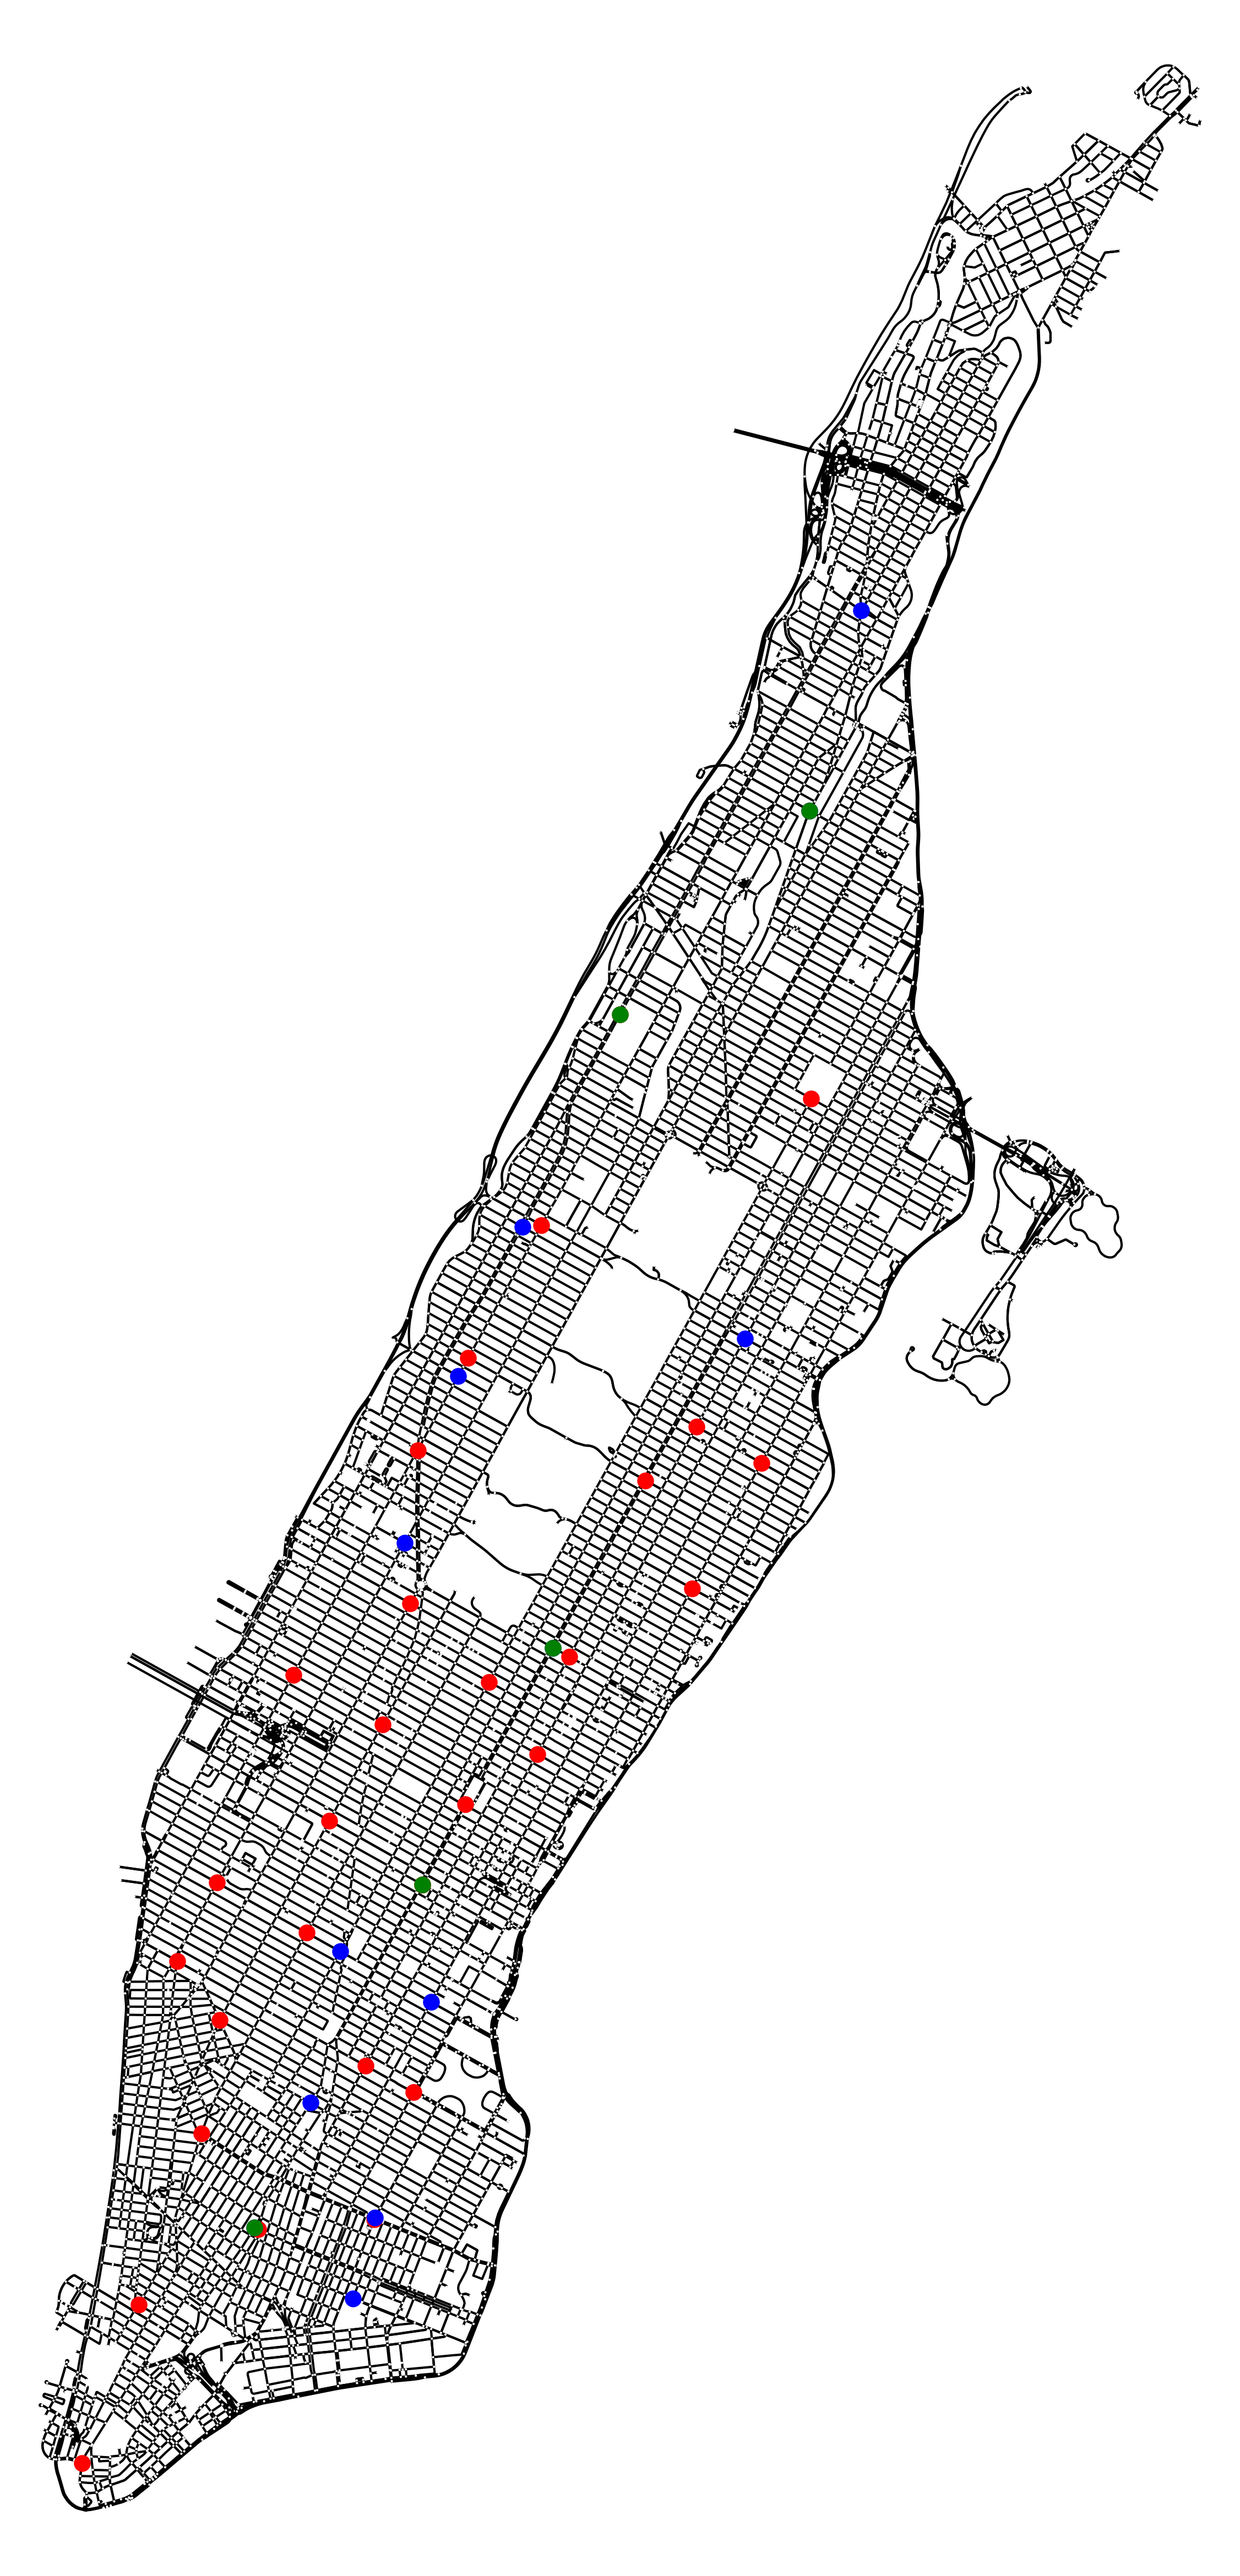
\includegraphics[width=0.45\textwidth]{img/new_york_vanilla_info.png}};
	 					\node[right=0.1cm of left, scale=2] {$\Rightarrow$};
	 					\node (right) at (4,-1) {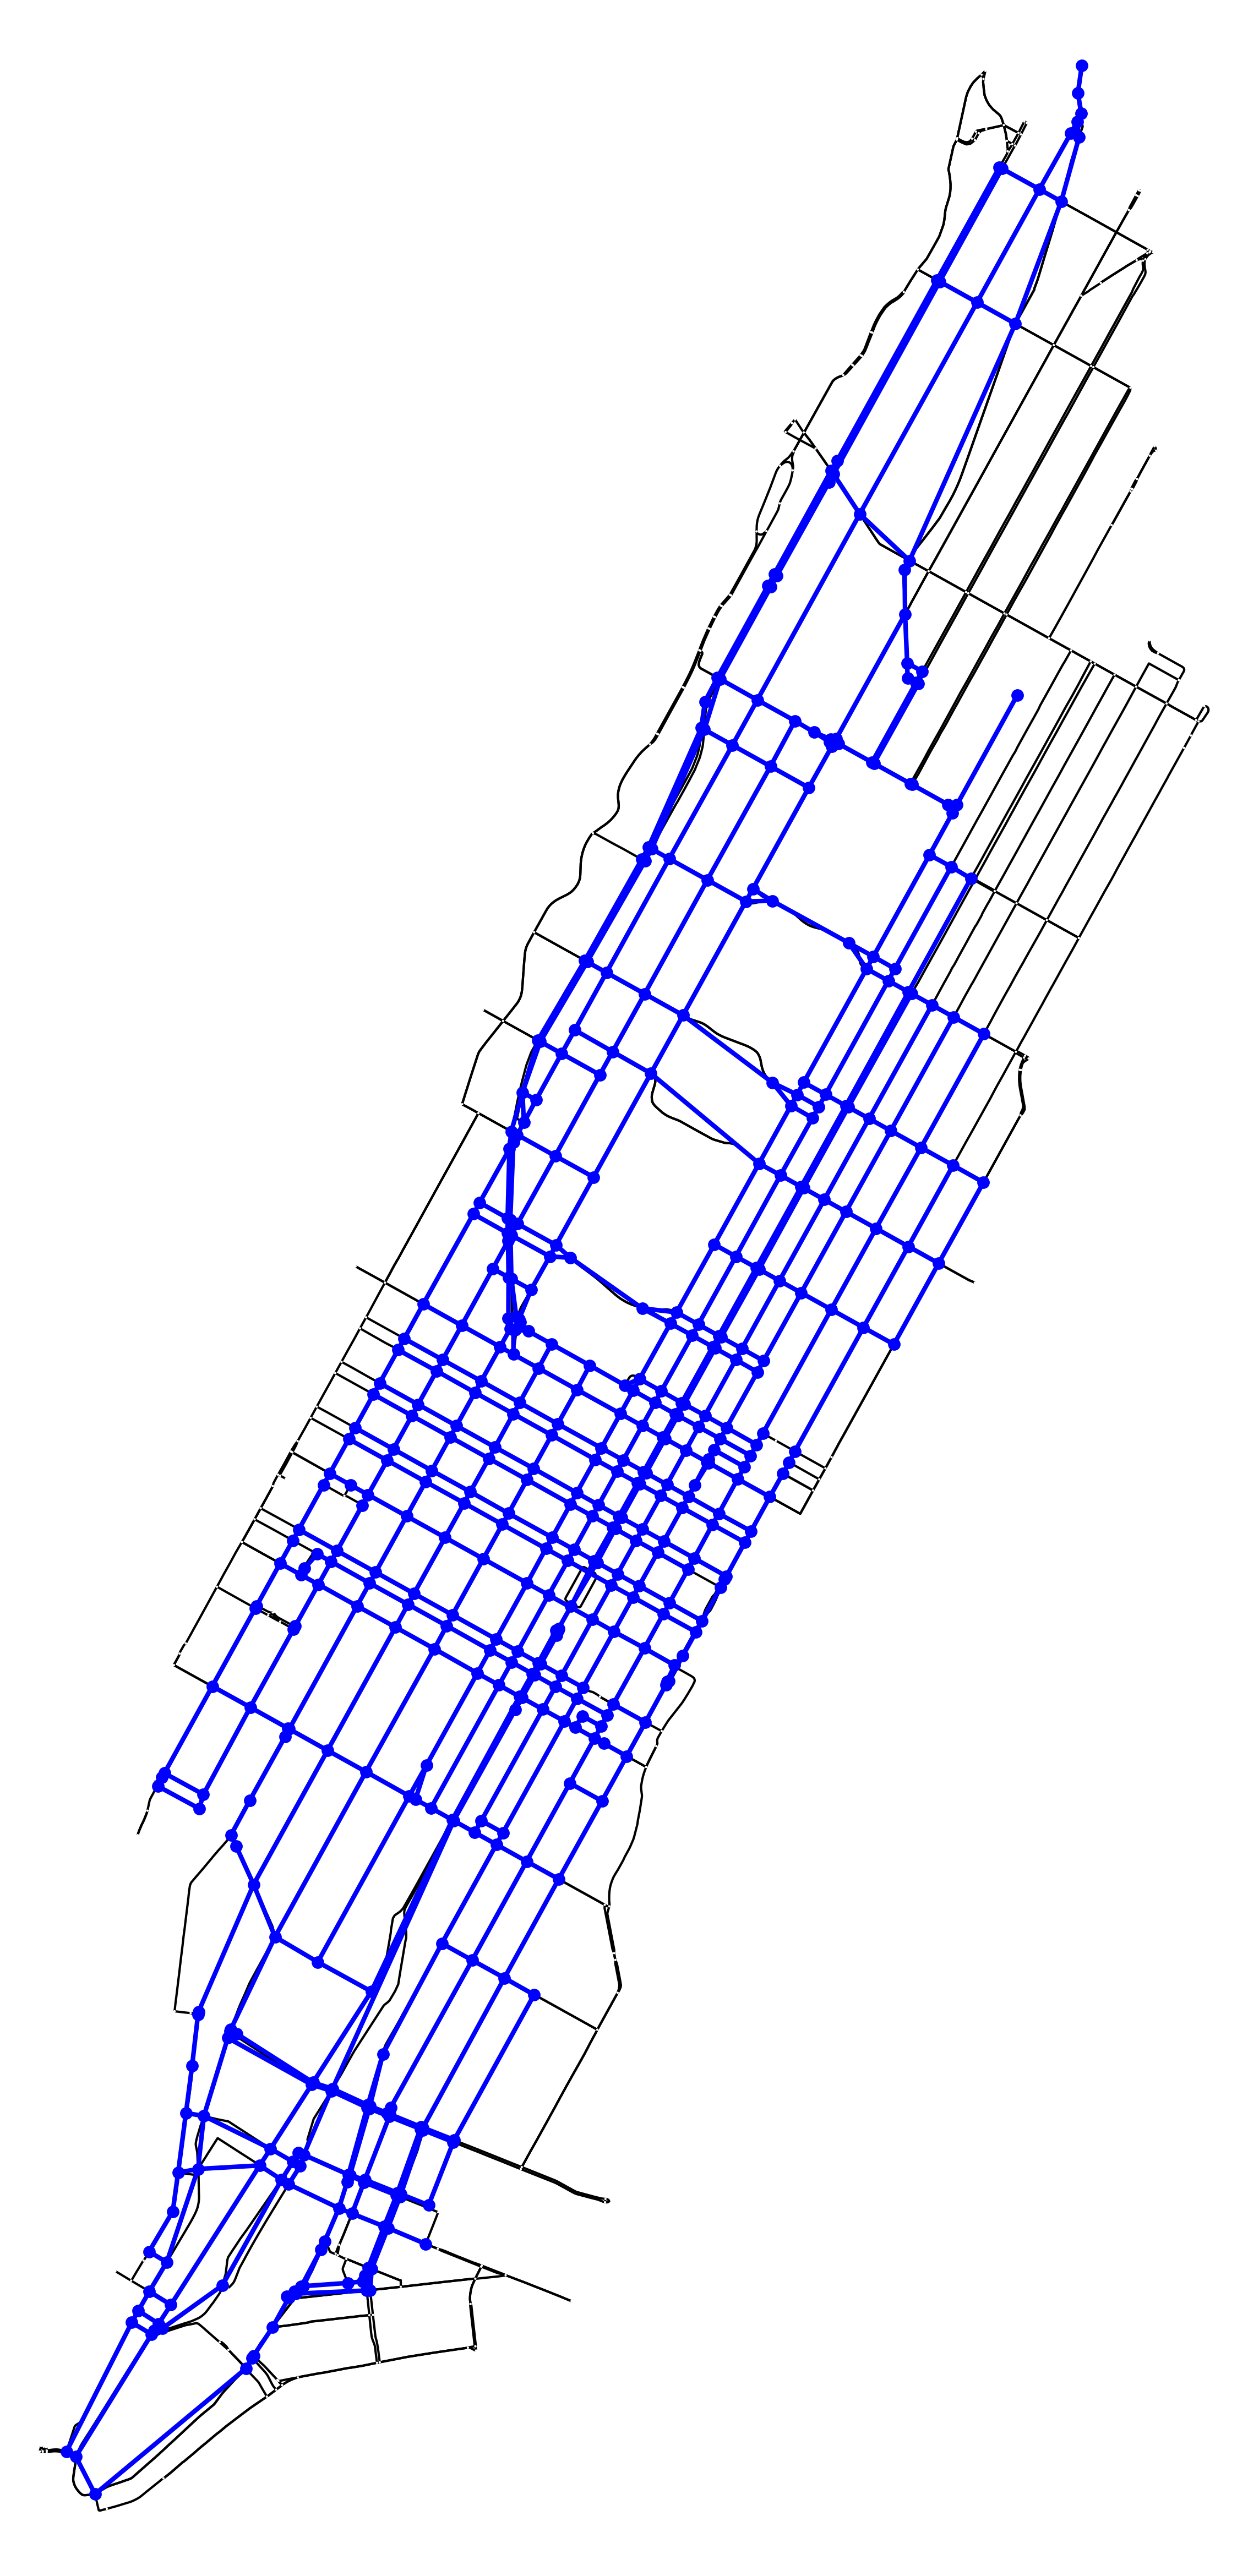
\includegraphics[width=0.45\textwidth]{img/new_york_simplified_roads.png}};
	 				\end{tikzpicture}
	 			\end{figure}
	 			\vspace{0.5cm}
	 		\end{column}
	 \end{columns}
\end{frame}


% ==================///==================///==================///
\begin{frame}{Evaluation}
	\hspace{0.5cm} Promising results, but interrogatives are left open. 
	\vspace{0.5cm}
	\begin{columns}
		\begin{column}{0.35\textwidth}
			
			\begin{itemize}
				\item[+] Solves all the challenges
				\item[+] Reduced computation thanks to a clever rebalancing formulation
				%\item[+] Numerically optimal solutions
				\item[+] Flexible and Modular model
			\end{itemize}
		\end{column}
		%%
		\vline
		\hspace{0.8cm}
		\begin{column}{0.4\textwidth}
			\begin{itemize}
				\item[-] Congestion model is highly simplified
				\item[-] Suffers large networks 
				%\item[-] Not suitable for real-time 
				\item[-] Does not gain insights on the future
			\end{itemize}
		\end{column}
	\end{columns}
\end{frame}